\documentclass[a4paper,11pt]{report}

% Paquetes de idioma y codificación
\usepackage[utf8]{inputenc}
\usepackage[T1]{fontenc}
\usepackage{graphicx}
\usepackage{hyperref}
\usepackage{amsmath, amssymb}
\usepackage[numbers]{natbib}
\usepackage{listings}
\usepackage{geometry}
\usepackage{float}
\usepackage{caption}
\usepackage{titlesec}
\titleformat{\chapter}[hang]{\normalfont\huge\bfseries}{\thechapter.}{1em}{}
\setcounter{tocdepth}{3}
\usepackage{booktabs}
\usepackage{alltt}




% Configuración de márgenes según las especificaciones
\geometry{
    top=1in,
    bottom=1in,
    left=1.25in,
    right=1.25in
}

% Fuente Arial 11pt
\renewcommand{\familydefault}{\sfdefault}

% Espaciado de línea de 1.5
\renewcommand{\baselinestretch}{1.5}

% Configurar numeración de páginas
\pagenumbering{arabic}

% Configuración de pies de figura y tablas
\captionsetup{
    font=small,
    labelfont=bf,
    justification=centering,
    singlelinecheck=false
}

\title{\textbf{Comparative Study of Delaunay Path Planner and RRT* for Path Planning in Autonomous Racing}}
\author{Rodrigo Carri\'on Caro}
\date{April 4th, 2025}


\begin{document}

\maketitle
\tableofcontents
\newpage

\chapter*{Glossary}
\addcontentsline{toc}{chapter}{Glossary}
\begin{itemize}
    \item \textbf{RRT} – Rapidly-Exploring Random Tree, a path planning algorithm designed to efficiently explore large search spaces.
    \item \textbf{ROS2} – Robot Operating System 2, a modular framework for developing robotic software systems.
    \item \textbf{YOLO} – You Only Look Once, a deep learning architecture for real-time object detection.
    \item \textbf{mAP} – Mean Average Precision, a metric used to evaluate the accuracy of detection models.
    \item \textbf{IoU} – Intersection over Union, a metric that measures the overlap between predicted and actual bounding boxes.
    \item \textbf{YOLOv5, YOLOv8, YOLOv11} – Specific versions of the YOLO model with different architectures and improvements.
    \item \textbf{mAP@50, mAP@50–95} – Variants of mAP that evaluate precision at different IoU thresholds.
    \item \textbf{OBRA} – \textit{Oxford Brookes Racing Autonomous}, the university team developing autonomous competition vehicles.
    \item \textbf{SLAM} – Simultaneous Localisation and Mapping, a technique used to build a map of the environment while tracking the agent’s position within it.
    \item \textbf{MPC} – Model Predictive Control, an advanced control strategy used to optimise vehicle performance under constraints.
\end{itemize}

\newpage

\chapter*{Abstract}
Autonomous racing presents a specific challenge to robotics in the field of high-performance 
decision-making under real-time and dynamically changing environments. Path planning, as a core 
component of the autonomous stack, must balance computational efficiency and adaptability with optimality of the trajectory. 
This project addresses these requirements through the design and testing of a modular path planning system for the Oxford Brookes Racing Autonomous (OBRA) car.

To begin with, the Delaunay triangulation-based planner used last year was overhauled for improved 
readability, efficiency, and stability. Next, two new RRT* (Rapidly-exploring Random Tree Star) algorithm 
implementations were independently coded from scratch: one for midline trajectory consistency and another for racing 
performance with forward-biased sampling and spline-based smoothing. All planners were tested over numerous laps and scenarios 
in a realistic Unity-based simulator, allowing for a detailed, metric-based comparison.

The results of this work comprise the technical foundation for the deployment of an optimised RRT* 
planner on the OBRA vehicle this year. Furthermore, the modular strategy and testbed enable generalisability 
to other autonomous vehicle programs in which adaptive, high-performance planning is required.

\chapter*{Acknowledgements}
\addcontentsline{toc}{chapter}{Acknowledgements}

I would like to express my sincere gratitude to my supervisor, \textbf{Muhammad Younas}, 
for his guidance, support, and continuous feedback throughout this project. 

My sincere thanks to the \textbf{Oxford Brookes Racing Autonomous (OBRA)} team for fostering a 
collaborative and technically driven environment. I am particularly grateful to \textbf{Aduén Benjumea} and 
\textbf{Mihir Gohad} for their leadership and guidance throughout the year.

Special thanks to \textbf{Sebastian Donnelly} for his continuous support and practical insight, 
and to \textbf{Dorian Amaritei} for his key contributions to the Delaunay planner’s optimisation.

I would like to also show my appreciation towards \textbf{Pablo Gutiérrez}, whose expertise in simulation was essential for validating the planners under realistic conditions.

\newpage
\chapter{Introduction}
\section{Background}
In the domain of autonomous racing, safe and fast racing relies on efficient and adaptive trajectory planning. 
Neural networks and geometric planners have traditionally been used, but they often fail to provide the responsiveness needed for rapidly changing environments.
The Delaunay path planner, developed within Oxford Brookes Racing Autonomous (OBRA), offers deterministic and structured trajectories, though it requires further optimisation under dynamic conditions.

To deal with these issues, this project presents a comparison between two very different planning styles: the Delaunay path planner and the Rapidly-exploring Random Tree (RRT/RRT*) algorithm \cite{reference1}. 
RRT algorithms are well known for their technique to search complex, high-dimensional areas quickly so they can be used in settings where fast changes are needed \cite{reference2}. Delaunay triangulation methods 
on the other hand could provide gentler paths at a lower cost when the environment is predictable.

The main objective of this project is twofold: complete the development of an RRT-based planner for OBRA’s system and compare its performance rigorously with the Delaunay planner that exists. 
The evaluation metrics are adaptability, route quality, and computation time in static and dynamic simulated environments. This comparison will give a clear idea about 
strengths and weaknesses of each approach, which will ultimately assist the OBRA team in choosing the best appropriate solution for competitive racing scenarios.

\section{Aim}

The aim of this project is to improve the current Delaunay and to develop the RRT* algorithm. 
Both will be implemented within OBRA's system to enhance route planning capabilities and performance in dynamic racing environments. 
Additionally, this project aims to compare the performance of the RRT* algorithm with the  Delaunay path planner to 
determine the most efficient and adaptable solution. This will enhance the car's route 
planning capabilities and optimise its performance in dynamic racing scenarios.

\section{Objectives}
\begin{itemize}
    \item To conduct a comprehensive study of path planning techniques used in autonomous vehicle 
    navigation, analysing their advantages, limitations, and applications in high-speed racing scenarios.
    \item To optimise the existing Delaunay-based path planner that enhances adaptability, 
    computational efficiency, and trajectory smoothness in dynamic environments.
    \item To develop a new RRT algorithm from scratch for real-time path planning 
    in autonomous vehicles, ensuring compatibility with the OBRA car's ROS2 framework.
    \item To enhance the RRT algorithm by integrating RRT*, improving its 
    ability to generate efficient and dynamically adaptable routes.
    \item To validate both the optimised Delaunay and RRT* algorithms in a controlled simulation 
    environment using Unity, testing their performance under varying racing conditions.
    \item To conduct a detailed comparative analysis of the optimised Delaunay and RRT* algorithms, 
    evaluating key performance metrics such as computation time, path efficiency, adaptability to dynamic obstacles, and robustness in high-speed scenarios.
    \item To identify and address potential limitations of each algorithm, 
    proposing refinements or hybrid approaches that could further enhance their performance.
    \item To integrate the most effective path planner into the OBRA team's autonomous racing pipeline, 
    ensuring real-world applicability and alignment with competition requirements.
\end{itemize}


\section{Product Overview}
\subsection{Scope}
The objective of this project is to develop and optimise two new path planners for autonomous racing \cite{reference4}:
\begin{itemize}
    \item Optimised Delaunay Path Planner – A modified version of the traditional 
    Delaunay-based planner, improving its efficiency and adaptability for dynamic racing environments.
    \item RRT* – An enhanced Rapidly-exploring Random Tree algorithm that generates 
    smoother and more efficient paths by reducing randomness and refining route selection \cite{reference3}.
\end{itemize}
Both planners will be developed in Python to ensure seamless integration with the ROS2 framework 
used by the OBRA autonomous system. The validation process will be carried out in simumalation environments using Unity, 
allowing for thorough evaluation before potential real-world deployment.

Once developed, both planners will be evaluated side by side to determine which gives 
better success in terms of flexibility, computational effectiveness, and path smoothness under high-velocity, dynamic conditions.

\subsection{Audience}
The project is primarily aimed at the OBRA team. They will be the ones using the 
algorithms to improve the car's performance in competitions. Additionally, it is a 
relevant project for the academic community, particularly in the fields of robotics and 
autonomous vehicles. From a professional perspective, the project holds significance 
for industry professionals interested in the implementation of path planning techniques 
in autonomous systems

\newpage
\chapter{Background Review}
\section{Existing approaches}
Currently, the OBRA autonomous car uses a Delaunay path planner. This planner is functional in 
controlled situations but have limitations when it comes to adapting to rapid changes 
in the environment.   
For such cases, the RRT algorithm is ideal. It efficiently explores large search spaces 
in real time. RRT* is its more optimised version, which improves the quality of the routes, 
making them shorter and more efficient \cite{reference5}. By implementing RRT* from scratch, I aim to 
enhance the flexibility and optimisation of the car's path planning system.

\section{Related Literature}

A review of the literature indicates a wide range of studies investigating RRT*, its optimisations, and associated applications in autonomous navigation.

Zhao et al. (2021) suggested an extension to bidirectional RRT*, enabling not only reduced paths but also faster convergence. Their findings, though, exist mostly in the realm of static environments and therefore restrict their direct use to real-time racing environments' dynamic requirements. In spite of this, the computational advantages obtained there remain quite relevant for the RRT* implementation implied in this work.
\cite{reference5}

Gasparetto et al. (2015) provide a pioneering compendium describing traditional motion planning paradigms, such as Roadmaps, Cell Decomposition, and RRT. Although their treatise is mainly focused on static and industrial settings, their theoretical framework regarding RRT offers detailed background information to apply such techniques to high-speed racing settings. \cite{reference6}

Wang et al. (2022) has proposed an underground autonomous vehicle RRT* algorithm optimisation with step size and turn angle constraint. Though the boundaries of their interest are underground, floorless, the restraint focus planning aspects are relevant for platforms like OBRA that use Ackermann steering like a car.
\cite{reference7}

Sánchez-Ibáñez et al. (2021) centered on the categorisation of algorithms applied to path planning based on their applications, primarily bounded within controlled environments. Nonetheless, their taxonomy supports the selection rationale of why RRT* was chosen over A* or Dijkstra in dynamic racing environments.
\cite{reference8}

Messer et al. (2022) outline the use of RRT* algorithms with Python to plan operations for concentric tube robots. Their work enhances the use of Python for this project and also its integration with ROS2-based systems, which is essential for this project's fulfillment.
\cite{reference9}

Kolski et al. (2006) explain hybrid methods of planning in dynamically changing environments. They write about navigation through moving obstacles and highlight the factor of real-time changeability, a significant factor in autonomous racing. Their work is implemented for developing the criteria for evaluation taken up in this research.
\cite{reference10}

Lei et al. (2025) introduce RRT* ASV, an RRT* optimised for Ackermann steering vehicles. This is of specific interest to OBRA, which requires related planning modifications due to its kinematic limitations. This work drew attention to taking vehicle dynamics into account in planning trajectories.
\cite{reference11}

Machavaram (2025) discusses aspects of adaptive Neuro-Fuzzy control systems for path planning. While they do not link the work to RRT* explicitly, the focus on decision-making in the presence of changing conditions leaves open the possibility of adaptive replanning in the future.
\cite{reference12}

Yoon, Y., and Jo, A. (2025) suggest an adaptive with location of obstacles path sampling approach using neural networks. Their solution is thinking about the problem in a completely different way, but a reminder of the value of adaptive and hybrid solutions. \cite{reference13}

Yan et al. (2025) discuss the problem of path planning with city traffic constraints. According to their work, the benefit of active, real-time planning is revealed, which this project tries to achieve in competitive autonomous navigation.
\cite{reference14}

All of these works help validate an RRT-based planner for this task. Most of the work aims for a controlled or domain-restricted environment; nonetheless, some propose transferable optimisation, constraint handling, or real-time adaptation strategies. The literature also allows for several future directions, including combining RRT with data and learning-based heuristics and cost functions for dynamic replanning.


\subsection{Originality}
Though most of the studies that were reviewed concentrate on optimising RRT* for a static or bounded environment \cite{reference3, reference4, reference5}, 
the distinguishing factor of this project was the use of a custom built RRT* planner for high-speed autonomous racing. 
This project stands out because it integrates a new RRT* implementation into an actual simulation of the Silverstone racing 
circuit.

Also, the developed variant of RRT* was implemented with Python from scratch and integrated into ROS2, making 
it compatible with the OBRA software. These claims regarding integration are verifiable because the performance 
metrics like lap time, trajectory smoothness, and stability measured autonomously are no longer theoretical, 
but rather grounded in a real-world scenario using an autonomous racing vehicle \cite{reference2}.

Additionally, this project incorporates a comparative approach based on simulation exercises by testing 
the planner’s performance over extended sessions, including 20 consecutive laps, to evaluate its reproducibility 
and its range of variations. Such a detailed evaluation under highly controlled racing conditions is what sets the 
project apart from generic applications in robotics and advance the understanding of sampling based algorithms.

\chapter{Methodology}
\section{Application of Agile Methodology}

The Agile methodology is based on the principles of iterative development, 
where requirements and solutions evolve through collaboration between self-organising \cite{reference21, reference22}.

Agile was preferred over traditional models due to its iterative and adaptive development cycles, 
which are more suitable for research-based projects. Unlike rigid and linear frameworks such as Waterfall \cite{reference23}, 
Agile enables continuous feedback, evolving requirements, and flexible task reallocation. 
This proved especially useful in a context where both technical implementation and experimental testing evolved throughout the project lifecycle.

In the context of this project, Agile proved to be especially suitable due to several key characteristics:

\begin{itemize}
    \item The project required the development and refinement of multiple algorithms 
    (Delaunay and RRT*) in parallel, which would be difficult to coordinate under a sequential methodology.
    \item Several unknowns emerged throughout the project, such as ROS2 integration issues, 
    simulation-specific bugs \cite{reference15}, and evolving optimisation goals. Agile allowed reallocation of effort 
    based on the results of each sprint.
    \item Frequent testing and simulation were essential for validating progress. 
    Agile naturally supports test-driven development and iterative validation \cite{reference22}, which 
    aligns well with the experimental nature of this work.
    \item The dual focus on technical development and research (e.g., literature review, algorithm design, integration testing) 
    required a dynamic workflow where tasks could evolve and overlap.
\end{itemize}

\section{Iteration Breakdown}

Based on the Agile model, the development process was divided into five major phases, each building upon the outcomes of the previous one \cite{reference21, reference22}. 
The phases were structured as follows:

\begin{figure}[H]
    \centering
    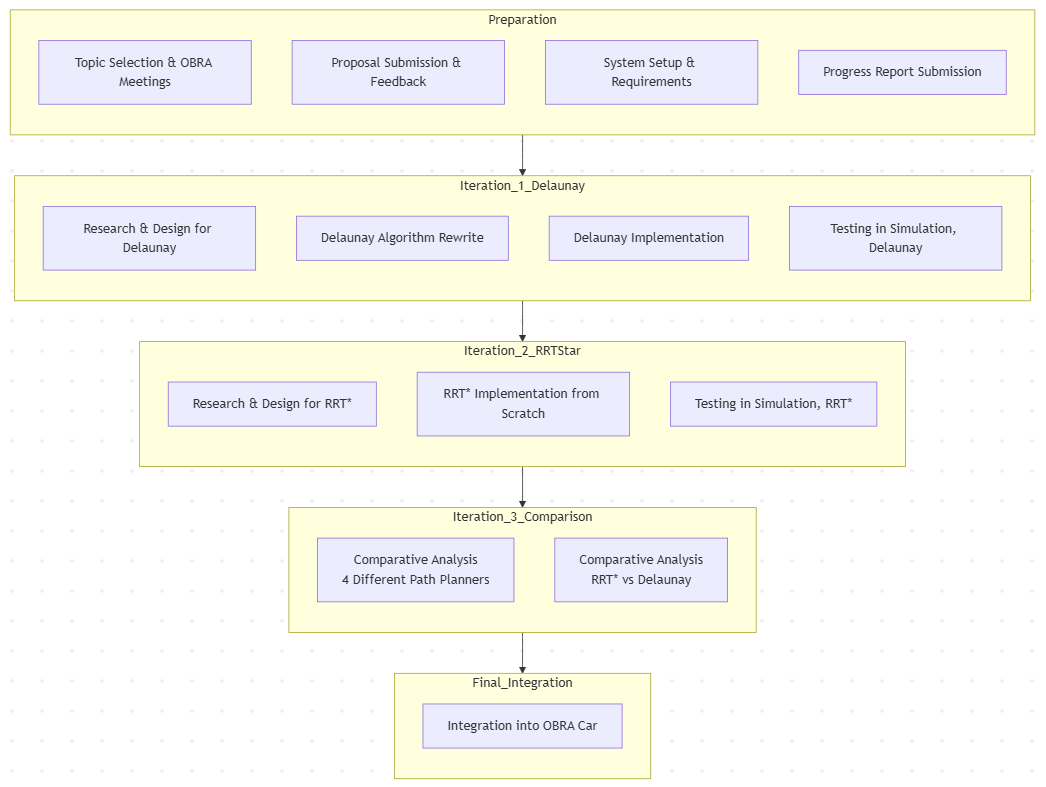
\includegraphics[width=1\textwidth]{Images/methodology.png}
    \caption{Modular Development Flow — Iterative Structure of Project Phases}
    \label{fig:methodology_diagram}
\end{figure}

\begin{itemize}
    \item \textbf{Preparation Phase:} Definition of the project topic, coordination meetings with OBRA, and writing of the initial proposal. Tools and systems such as Ubuntu, ROS2, Unity and Foxglove were installed and configured for development and testing purposes \cite{reference15, reference16, reference17, reference20}.
    
    \item \textbf{Iteration 1 – Delaunay Optimisation \& Rewriting:} Analysis of the Delaunay triangulation method. The original algorithm was refactored and optimised to enhance stability and performance. The implementation was validated in the Unity simulation environment.
    
    \item \textbf{Iteration 2 – RRT* Development from Scratch:} A full implementation of RRT* was carried out from first principles. Theoretical foundations were studied, followed by coding and simulation-based evaluation to validate its performance under similar conditions.
    
    \item \textbf{Iteration 3 – Comparative Analysis:} A thorough comparison was conducted between the RRT* and the optimised Delaunay planner, including a side analysis of alternative planners developed throughout the project. Metrics such as path smoothness, time efficiency, and adaptability were evaluated in controlled simulation runs.
    
    \item \textbf{Final Validation and Integration:} The best-performing path planner at the end of this season will be integrated into the OBRA autonomous car. Specific attention will be given to hardware limitations, communication with ROS2 nodes, and real-time inference compatibility \cite{reference15, reference16}.
\end{itemize}

\section{People Involved}
Throughout the project, collaboration with the Oxford Brookes Racing Autonomous (OBRA) team was essential. 
Their input helped define the system requirements, particularly regarding the car's ROS2 integration and simulation constraints \cite{reference16}. 
Regular meetings and feedback from OBRA members guided the practical implementation and ensured that the developed algorithms aligned with the team's real-world racing needs.

\chapter{Technology}
\section{Implementation Tools and Resources}

To ensure smooth implementation and testing of the project, we emphasised the use of primary technologies and tools. 
Python serves as the primary programming language for implementing the algorithms and system logic in this project. 
Python is used to develop the path-planning algorithms, integrate them into ROS2,
and manage the necessary data processing tasks. Its many libraries, along with its useable features in machine learning 
and robotics frameworks, enable it to be ideal for rapid prototyping and testing purposes.

To aid with robot integration, we use ROS2 (Humble) which enables easy transmission between parts of the 
autonomous system \cite{reference15}. ROS2 takes care of real-time control, path planning and processing of sensor data, which 
guarantees that all modules are in coordination with one another. The role of the middleware in taking care of 
many nodes is vital in real-time decision-making in the autonomous vehicle.

Ubuntu 22.04 was selected due to its stability and compatibility with ROS2, Python-based frameworks, 
and simulation tools such as Unity and Foxglove \cite{reference15, reference17}. For the robotic frameworks that are required for this project, 
Ubuntu provides support and there is a large community available for help and further enhancements.

For version control purposes, the code modification is stored altered on the central repository, 
Git and Gitlab \cite{reference24}. Previous development on OBRA´s GitLab is stored in the OBRA workspace.

\section{Workspace}
\subsection{OBRA WS}
The Oxford Brookes Racing Autonomous (OBRA) workspace arranges modules in a top-down manner of
system architecture. Every major autonomous pipeline has a component developed by a subteam.
This allows parallel development while making sure that everything integrates well with the system.
Figure~\ref{fig:software_architecture} gives a top-down view of the autonomous stack,
showing the data flow between the modules and how they interact with real-world and
simulated environments.

The system is divided into key subsystems; Sensors Suite, Perception, Localisation \& Mapping,
Trajectory Planning, and Controls. Each subteam is responsible for the development, testing, and integration
of one of these subsystems and they work collaboratively through shared interfaces and simulation environments.
This architecture should not only support scalability and maintainability but also show the nature of the team,
coming from different expertise related to computer vision, robotics, AI, and control systems.

Development and testing are done in real as well as simulated environments.
The simulation setup models the track conditions such that it reflects the vehicle’s behavior
under any condition of the track. This provides a safe and agile way to confirm that the
improvements work before the physical car is given these improvements.


\begin{figure}[H]
    \centering
    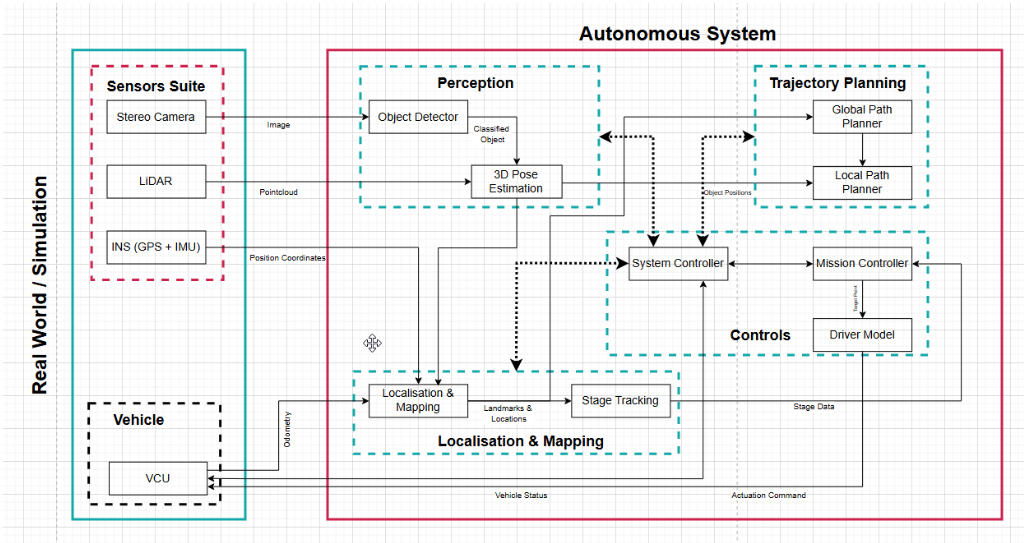
\includegraphics[width=0.95\textwidth]{Images/SoftwareArchitecture.png}
    \caption{Autonomous System Architecture — OBRA workspace modules and interfaces.}
    \label{fig:software_architecture}
\end{figure}

\subsection{ADS-wsgraph}
To visualise the structure of the OBRA ecosystem, we can execute the following command in the Ubuntu terminal:
\begin{verbatim}
rqt_graph
\end{verbatim}

This command shows a graph of the ROS2 nodes and topics running.
To generate a graph similar to Figure \ref{fig:obra_graph}, the simulator and the OBRA workspace must be correctly configured and actively running.

\begin{figure}[h]
    \centering
    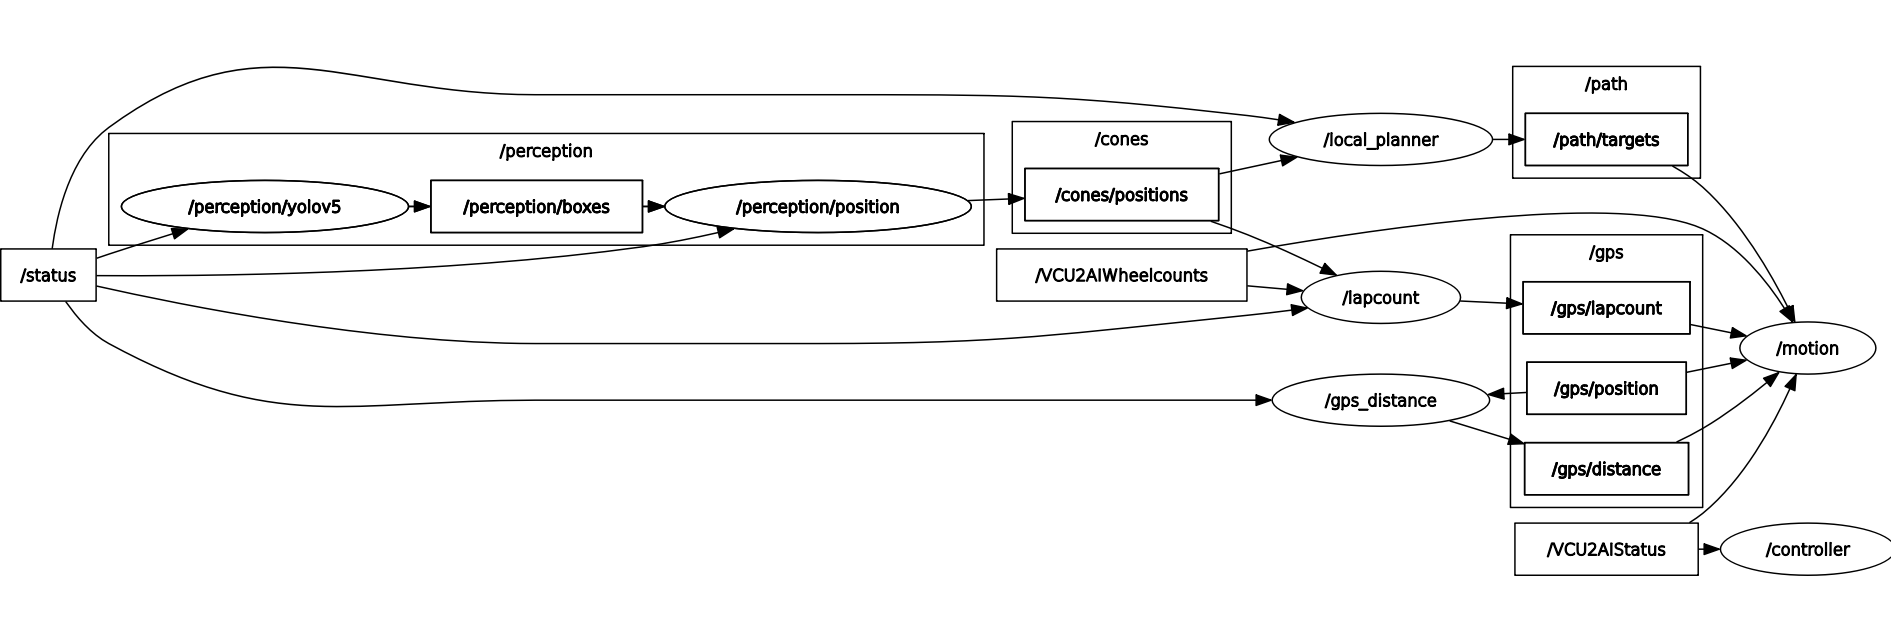
\includegraphics[width=\textwidth]{Images/wsgraph.png}
    \caption{Ecosystem of nodes and topics in OBRA generated with rqt\_graph}
    \label{fig:obra_graph}
\end{figure}

The OBRA workspace comprises several nodes which interact via ROS2 topics so as to enable communication 
between different modules of the autonomous system \cite{reference15}. In the graph that \texttt{rqt\_graph} produces, 
we can see how the different components are laid out and how they communicate.

The \texttt{/status} node gives the system info and links with other prime modules. 
Inside the feel setup, the \texttt{/perception/yolov5} node takes pictures and forms bounding boxes, 
which go to \texttt{/perception/boxes} and then changed to positions through \texttt{/perception/position}. 
This data is used by other modules like path planning and localisation.

Data regarding the position of cones is routed through the topic \texttt{/cones/positions}; 
this is data that the module uses to make decisions about its routes (\texttt{/local\_planner}) and 
how many laps have been completed (\texttt{/lapcount}). The proper operation of the system also requires 
data from the localisation module pertaining to \texttt{/gps/lapcount}, \texttt{/gps/position}, 
and \texttt{/gps/distance} at its disposal to make fully informed decisions about what is required to enable a vehicle to drive itself.

Then, the control unit collects all that data and sends it to /motion so that the car can drive itself. 
The talk between these parts makes sure the right way the system works in a pretend setting or in the actual vehicle.

The following subsections describe the various system modules in detail:

\subsection{Perception}

Perception is the entry point of the autonomous system. Computer vision is used to process images 
from our stereo camera, the Zed 2i, and the Livox HAP LiDAR \cite{reference27}. The detection of cones is handled through 
the YOLO neural network which takes images from the left channel of the camera to infer the position of 
cones on a 2D map. Depth perception from the camera is handled by taking into account the bounding boxes 
from both camera channels and comparing the two received frames to estimate a distance to an object 
getting a midpoint for them to estimate distance. The most suitable base suitable model from Ultralytics 
was YOLOv11 Nano, due to having the fastest inference speed of the offered base models. Detection of 
small objects such as cones at a distance is challenging due to the resolution limitations of the camera. 
This led to modifications on the base YOLOv11 neural network to increase its accuracy to detect small objects, making use of the YOLO-Z approach \cite{reference26}.

The perception system also makes use of LiDAR in tandem with computer vision techniques. 
LiDAR works along the depth perception model from the Zed Camera to give an accurate distance 
estimation of the cones in the path of the vehicle, through point cloud data. The Livox HAP LiDAR 
also has a detection range of 150 meters. This enables the system to map far away cones, which the 
object detector and the camera would not be able to detect confidently due to resolution limitations 
which makes the color of the cones indistinguishable at extreme distances. This level of mapping is needed 
for SLAM and Trajectory Planning as the position of the cones are placed on a 3D map used by both of these systems \cite{reference27}.

\subsection{Localisation \& Mapping}
Simultaneous Localisation and Mapping (SLAM) is the module in which an agent constructs an understanding 
of a previously unexplored environment while simultaneously estimating its own position within the environment. 
Due to the inherent uncertainties in the sensors and actuators, SLAM is inherently probabilistic and combines the 
two key tasks: localisation which involves estimating the agent's own position based on the existing map and mapping 
which entails creating a map given an accurate position \cite{reference6}. The current SLAM module makes use of the IMU data along with the 
GPS and wheel speed sensor, to enhance the accuracy and reliability of both localisation and mapping \cite{reference27}. 
The inertial measurement unit (IMU) provides data for the agent’s orientation allowing for real time 
adjustments to its estimated position. The GPS provides data as a global reference point which is useful 
for the outdoor environments. The wheel speed sensors aid in odometry calculations by tracking all the tracking 
distances traveled. By integrating these sensors, the SLAM module effectively reduces the uncertainties and improves 
the reliability of the generated map allowing the agent to navigate the environment with greater precision.

To complement SLAM, additional systems are implemented for tasks like map cleanup, clustering, 
or loop-closure adjustments based on map conditions. In events where a prior map is provided, the 
full SLAM system is still launched with a preloaded map to reflect changes in the environment in the system. 
For the acceleration event, SLAM faces limitations due to the uniform and repetitive pattern of a straight line 
of cones, which poses challenges for landmark-based systems. In such cases, focus shifts to an Inertial Navigation 
System (INS), which fuses global positioning with odometry data to measure task progress from the start point while 
using landmarks for local navigation \cite{reference25}. For unknown tracks, such as autocross and track drive, the SLAM system plays 
a critical role in tracking landmark positions to enable robust path planning and control. It also aids in lap 
counting and monitoring task progress. Specifically, during the track drive event, the SLAM system signals a successful 
loop closure at the end of a lap. This significantly reduces overall system uncertainty, allowing path planning and control 
systems to operate at higher performance levels with an extended estimate of the track beyond the exploratory lap. Currently, 
our system emphasises improving our localisation algorithm with a focus on EKF localisation.

\subsection{Path Planning}

The trajectory planning module takes on the essential task of planning a path that may be feasible and effective for 
the vehicle to travel the course based on the details supplied by the sight and location sub-modules. 
Acknowledging the fundamental uncertainties of the SLAM algorithms, notably in the initial mapping phase, the trajectory 
planning module will adopt a methodology that in the context of the race optimises performance and safety \cite{reference6}.

RRT* path refinement is gradually developed in the exploration of the environment, therefore, minimalising 
useless deviations and providing smoother, shorter trajectories. It is, therefore, more applicable in autonomous racing 
where the decisions have to be based on rapidly changing information \cite{reference3, reference4}. The flexibility of RRT* in unanticipated, time-varying 
track layouts greatly overshadows the capabilities of Delaunay, based on structured, well-defined conical distributions, 
hence making it an ideal choice for the application considered \cite{reference1}.

Furthermore, RRT* can exploit such sparsely and irregularly 
distributed cones more efficiently to keep the vehicle on a feasible path in all circumstances.

Delaunay builds non-overlapping 
triangles between detected cones to estimate track boundaries and then generates a valid path that the vehicle can take. 
Computationally, this efficient means a lot for structured layouts; ergo, it is less reliable in complex scenarios \cite{reference6}. 
However, this can be considered an effective contingency plan for it to be used in external constraints, RRT*, to keep the vehicle always having a place to go.


\subsection{Control}

The Control module is responsible for the implementation of advanced control strategies that optimise the performance of vehicles on track. 
One of the most powerful methodologies is the Model Predictive Control (MPC), which was selected for the OBRA 
autonomous race car because of its predictive capabilities, optimisation-based approach, and ability to handle 
constraints, unlike traditional controllers like PID. MPC optimises the car's trajectory over a prediction horizon, 
allowing it to anticipate future states and make optimal decisions at each time step \cite{reference25}.

MPC works by solving an optimisation problem at each step to find the best control inputs that will minimise 
the cost function. This cost function typically includes deviation from the desired trajectory, minimisation 
of control efforts and respecting dynamic constraints. It works with the inputs: that are circuit coordinates and vehicle dynamics 
(mass, inertia, tire stiffness), with MPC optimisation, that predicts vehicle motion, minimises trajectory deviation, 
and optimises control actions, and vehicle simulation that updates lateral forces and yaw rate via the Bicycle Model 
for real-time adaptation.


\subsection{Hardware and Sensors}

The system works on the premise that all required sensor equipment is housed within our Sensor Plate (SP). 
The SP runs on a limited 10A power supply which forces strategic choice of sensor hardware. 
The SP can be attached, removed and modified in a quick time. Ease of service has been considered with the 
body having various access points to ensure functionality.

The placement of each sensor equipment is determined to maximise the performance out of them while adhering 
to the regulations. The Livox HAP TX LiDAR is placed at the base of the SP and as far forward as allowed by the 
ADS-DV side view envelope to be able to detect the cones and have an unobstructed field of view \cite{reference27}. The Zed2i Camera 
is therefore put on top of the LiDAR to still be centered and field of view obstruction from the LiDAR is 
minimised by placing it as close to the side view envelope as possible. In addition, the dual GPS antenna setup 
is placed as far apart as the front view envelope allows for more error correction in the GPS drift.

The system is designed to work as a complete autonomous module via the addition of compute on the SP, 
this allows for easier installation and use on a variety of vehicles. This is made possible by the use of 
a CAN bypass which allows direct connection to the vehicle control unit.

To aid software development the team has developed a small scale platform which replicates the IMechE’s 
ADS-DV as accurately as possible. We call this the ADS-BV (Brookes Vehicle). This platform is ideal for rapid 
testing and troubleshooting issues in a small confined space where we are limited to 20 km/h. This has led to 
the development of OBRA-P01 which is the 2014 OBR chassis fitted for autonomous driving. This system works to mimic 
the ADS-DV and ADS-BV as closely as possible, both testing platforms use an EPAS Microsteer MGU steering motor to allow 
for autonomous steering \cite{reference28}. In terms of braking the systems differ. The ADS-BV uses a linear actuator to actuate the 
mechanical brake pedal and an electromagnetic EBS to ensure maximum safety. The braking system for OBRA-P01 uses the 
traditional hydraulic system merged with electronic actuators that create a BBW system for autonomous braking. Emergency 
braking is achieved by an “always on” system which locks the wheels when the system has no signal. Both testing platforms 
use identical CAN system construction and VCU architecture to the ADS-DV to ensure a seamless transition between the 3 platforms.


\section{Simulation and Testing Tools}

The simulation and testing phase plays a crucial role in validating the path-planning 
algorithms before deployment in the real OBRA autonomous vehicle. The core of the simulation 
environment is built using Unity, which provides a controlled and highly customisable setting 
where different track conditions, obstacles, and environmental variations can be modeled \cite{reference17}. Unity 
allows us to evaluate the performance of the algorithms under high-speed driving scenarios, tight turns, 
and unexpected obstacles, ensuring that the vehicle can navigate efficiently and safely.

To complement the simulation process, we use Foxglove for real-time visualisation and analysis of key 
system data. Since our project is built on ROS2 (Humble), Foxglove acts as an interface to monitor ROS2 
topics, displaying critical information such as vehicle state, planned trajectories, sensor readings, and 
dynamic obstacle detection \cite{reference20}. This visualisation is essential for debugging, performance assessment, 
and fine-tuning the parameters of our path-planning algorithms.

This simulation environment offers a critical development sandbox for validating the feasibility, responsiveness, 
and robustness of the planning logic before transitioning to physical deployment. The validation process is structured 
around a set of performance metrics, ensuring that each algorithm is assessed based on objective criteria. These metrics include:

\begin{itemize}
    \item Path efficiency: Measuring the distance and curvature of the generated trajectory.
    \item Computational speed: Evaluating how quickly the algorithm produces a valid path.
    \item Adaptability to dynamic environments: Testing how well the planner reacts to changes such as moving obstacles or shifting track conditions.
\end{itemize}

Once the simulations are completed, the results, including logs, performance data, and video 
recordings, will be stored in Google Drive for further analysis and comparison. This repository allows 
the team to track improvements over time and make data-driven decisions when optimising the algorithms.

By integrating Unity for simulation, Foxglove for real-time monitoring, and Google Drive for data storage, 
we establish a structured and efficient testing framework. This ensures that our path-planning algorithms are 
rigorously validated before integration into the OBRA vehicle, minimising risks and maximising system reliability.

\chapter{System Code Implementation}
This chapter gives the implementation details of the path planning system developed for the OBRA autonomous vehicle. 
It explains the structure of the codebase and the key scripts involved in addition to the design choices behind switching 
from a Delaunay-based planner to a more dynamic and adaptable implementation of RRT* \cite{reference6}. Each planner is described in terms of 
functionality, optimisations, and performance trade-offs. Version control strategy and development workflow is also included 
to reflect software engineering best practices \cite{reference18}.


\section{Path Planning Folder Structure}

To get the general outlook of the path planning directory, refer to the diagram in Figure
\ref{fig:path_planning_structure}. This organises different parts in charge of planning
the vehicle's path using either the Delaunay triangulation way or the RRT* algorithm.

\begin{figure}[h]
    \centering
    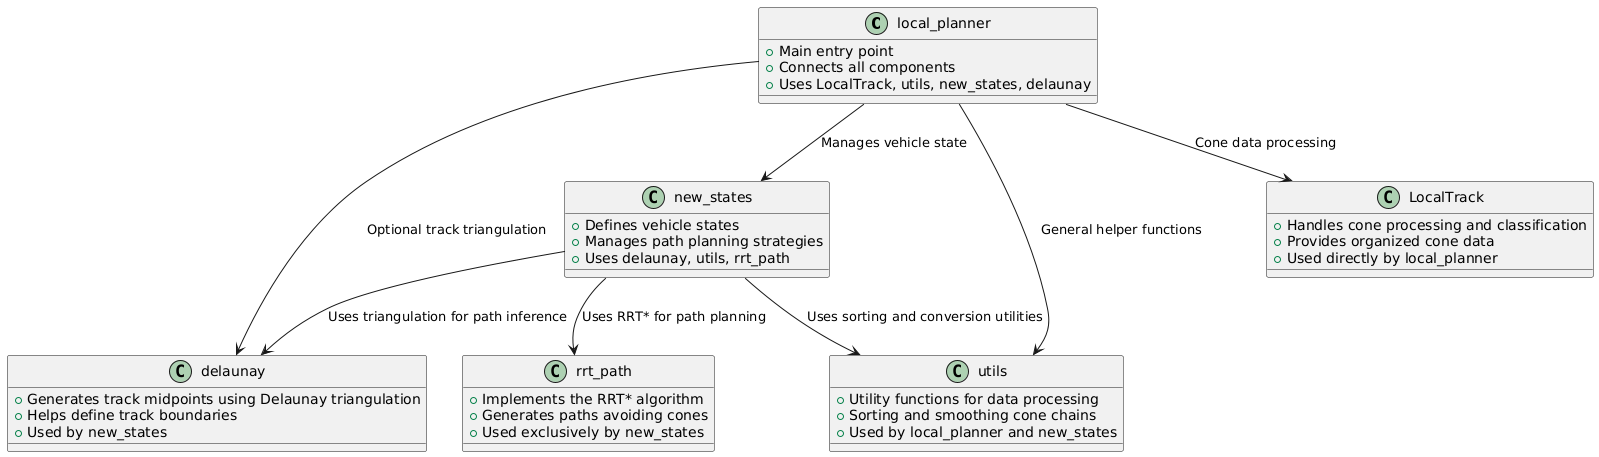
\includegraphics[width=\textwidth]{Images/local_planner.png}
    \caption{Path planning folder structure}
    \label{fig:path_planning_structure}
\end{figure}

The main entry point of the path planning system is the \texttt{local\_planner.py} script. This module connects all components and manages the overall planning process. 
Within \texttt{local\_planner}, the function \texttt{change\_state(self)} determines whether to use Delaunay or RRT* based on the detected environment. 
The selection is made using the following lines of code:

\begin{verbatim}
self.state = RRTStarState(self)  # Uses RRT* for path planning
self.state = Delaunay(self)      # Uses Delaunay for path inference
\end{verbatim}

\subsection{Local Planner (local\_planner.py)}
The \texttt{local\_planner.py} script is also responsible for subscribing to relevant ROS2 topics, processing incoming data, 
and determining the appropriate path planning algorithm. The script maintains real-time vehicle position 
updates and cone detection to adjust its planning method dynamically.

A key function in \texttt{local\_planner.py} is \texttt{change\_state(self)}, which decides whether to use the RRT* or Delaunay algorithm based on the available cone data:

\begin{verbatim}
def change_state(self):
    """
    Determines the path planning method based on detected cones.
    """
    if count_blue > 0 and count_yellow > 0 
    and count_blue + count_yellow > 3:
        self.state = RRTStarState(self)  
        # Selects RRT* when complex or dynamic scenarios are detected
    else:
        self.state = Delaunay(self)  # Defaults to Delaunay triangulation
\end{verbatim}

The function first verifies if both blue and yellow cones have been detected by the system.
If enough cones have been found, it picks \texttt{RRTStarState} since the RRT* algorithm is better for more complex,
dynamic paths. If fewer cones are found, it falls back to Delaunay triangulation; this track uses
precomputed midpoints for a path that is stable and well behaved.

\subsection{State Management (new\_states.py)}
The \texttt{new\_states.py} module defines the behaviour of different path planning strategies. 
It manages vehicle states and allows seamless switching between planning methods depending on the track conditions. 
The state management system is based on an abstract class \texttt{LocalPlannerState}, which enforces the implementation of a \texttt{plan\_path} method in all subclasses.

One of the primary states is \texttt{RRTStarState}, which utilises the RRT* algorithm for adaptive path generation:

\begin{verbatim}
class RRTStarState(LocalPlannerState):
    def plan_path(self):
        """Implements the RRT* algorithm for path planning."""
        try:
            # Ensure car position is defined
            if not hasattr(self.context, "car_position") 
            or self.context.car_position is None:
                print("Warning: `car_position` is not defined.")
                return self.context.last_path

            # Extract cone positions from the local track
            cones_blue = cones_to_tuple_list
            (self.context.local_track.blue)
            cones_yellow = cones_to_tuple_list
            (self.context.local_track.yellow)
            
            # Instantiate the RRT* planner
            rrt_planner = RRTStarPlanner(cones_blue, cones_yellow)
            
            # Generate the path using RRT*
            path = rrt_planner.plan_path(start=self.context.car_position, 
            goal=self.context.target_position)
            
            if path is None:
                print("Warning: RRT* did not find a path, 
                using last known path.")
                return self.context.last_path

            return path
        except Exception as e:
            print(f"Warning: RRT* encountered an error: {e}")
            return self.context.last_path
\end{verbatim}

This function first ascertains the position of the car.
It then extracts cone locations and passes them to the \texttt{RRTStarPlanner},
trying to compute an optimal path; if it doesn’t: the last successful path, to keep up the stability.

\subsection{Utility Functions (utils.py)}
The \texttt{utils.py} module provides helper functions for sorting cone data, smoothing paths, and handling data conversions.

\begin{verbatim}
def sort_cone_chain(cones):
    """Sorts cones into a continuous chain for path planning."""
    return sorted(cones, key=lambda c: c.x)
\end{verbatim}

By integrating these components, the path planning system dynamically selects the best 
algorithm for any given scenario.

\section{Initial Path Planner: Old Delaunay Implementation}

The OBRA self-driving car used a path finder at the start of FSUK 2024 that was based on Delaunay triangulation. 
This path planner had been made by the team over 2023 and 2024 and served as the foundation for autonomous navigation in the competition.
It used the blue and yellow cones to make a track edge and calculate a fine way through the middle points of the triangled shape. 
By using Delaunay triangulation, the planner gave a steady and known route, making sure the car could drive well. 
The first Delaunay-based way planner does not have flexibility in changing settings, since it depends on fixed triangulation of cones that were found. 
It has problems with not placing cones well, cannot manage quickly moving barriers well, and does not have way softening, resulting in suboptimal trajectories. 
Also, it does not optimise paths for minimal turns or distance. This implementation, while effective, had limitations in dynamic obstacle avoidance and adaptability, 
leading to further refinements in the next loop.

\section{Delaunay Path Planner Optimisation and Rewriting}

The Delaunay path planner was optimised so that there was a large reduction in complexity, making it more efficient and easier to sustain.
Before, there were more than 750 lines of code that formed the old implementation, and it heavily relied on using a complex graph-based approach 
to manage cone connections and extract midpoints.

An integral part of the new system is the \texttt{TrackNavMesh} class, which covers up the complexity of cone links by working with the Delaunay triangulation API 
directly from SciPy. Instead of manually managing graph structures to represent the track, \texttt{TrackNavMesh} internally handles the construction and traversal 
of Delaunay triangles. It also brings together rules for picking inner midpoints between cones of different colours, streamlining the overall path generation process. 
By wrapping up this logic, \texttt{TrackNavMesh} improves code modularity, while ensuring consistent and efficient triangulation results. 
Now, less than 250 new lines introduces a streamlined structure based on the \texttt{TrackNavMesh} class, which efficiently handles the Delaunay triangulation 
and simplifies the extraction of midpoints.


\begin{figure}[h]
    \centering
    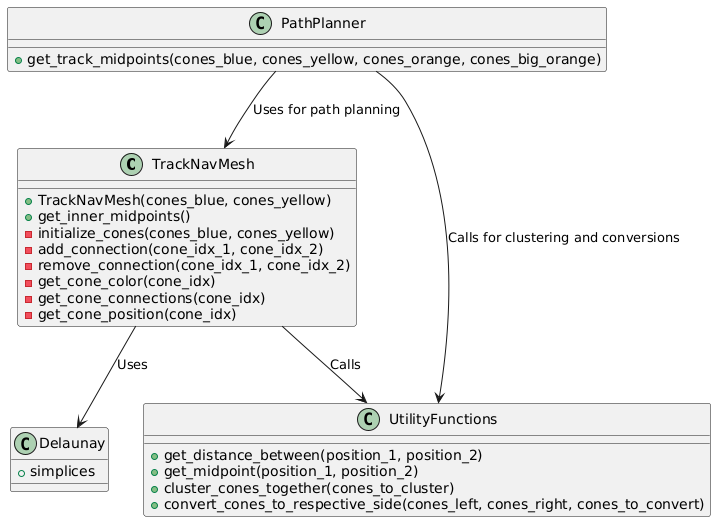
\includegraphics[width=\textwidth]{Images/delaunay.png}
    \caption{Optimised Delaunay Path Planning System}
    \label{fig:delaunay_optimisation}
\end{figure}

Figure \ref{fig:delaunay_optimisation} illustrates the restructured Delaunay path planner, highlighting key components and their interactions. 
The new system is structured around four main elements: \texttt{PathPlanner}, \texttt{TrackNavMesh}, \texttt{Delaunay}, and \texttt{UtilityFunctions}.

\subsection{Structural Simplification}

In the past, the planner used a graph that was manually managed to connect cones and find midpoints.
The new way of doing things makes these processes into TrackNavMesh, which directly uses the Delaunay class from SciPy to relate cones.

\begin{verbatim}
def get_inner_midpoints(self):
    result = []
    for triangle in self.delaunay.simplices:
        for cone_idx in triangle:
            for other_cone_idx in triangle:
                if self.get_cone_color(cone_idx) != 
                self.get_cone_color(other_cone_idx):
                    self.add_connection(cone_idx, other_cone_idx)
\end{verbatim}

By leveraging Delaunay triangulation directly, the systemeliminates the need for explicit connection handling, thereby reducing computational overhead.

\subsection{Efficient Midpoint Calculation}

Earlier, in midpoint calculations, there was a lot of nesting 
inside the loops, and filtering that caused more work.
The better way now just takes the midpoints from the triangulation directly and computes distances efficiently:

\begin{verbatim}
def get_distance_between(position_1, position_2):
    return math.hypot(position_1[0] - position_2[0], 
    position_1[1] - position_2[1])
\end{verbatim}

This approach consolidates distance calculations into a single function, removing unnecessary recalculations.

\subsection{Enhanced Cone Clustering for Smoother Paths}

The former system would merge closely positioned cones with
varying success, sometimes resulting in erratic paths. A new
implementation of the\texttt{cluster\_cones\_together}function will
guarantee that cones within a certain distance of each other are
always merged in a systematic manner.

\begin{verbatim}
def cluster_cones_together(cones_to_cluster):
    any_cone_within_max_cluster_distance = True
    while any_cone_within_max_cluster_distance:
        any_cone_within_max_cluster_distance = False
        for cone in cones_to_cluster:
            for next_cone in cones_to_cluster:
                if cone == next_cone: continue
                if get_distance_between(cone, next_cone) 
                < MAX_CLUSTER_DISTANCE:
                    cones_to_cluster.append
                    (get_midpoint(cone, next_cone))
                    cones_to_cluster.remove(cone)
                    cones_to_cluster.remove(next_cone)
                    any_cone_within_max_cluster_distance = True
\end{verbatim}

This method ensures smooth trajectories by preventing unnecessary sharp turns in the generated paths.

\subsection{Comparison of Old vs. New Implementation}

The table below highlights key improvements in the optimised Delaunay path planner:

\begin{table}[h]
    \centering
    \resizebox{\textwidth}{!}{
    \begin{tabular}{|l|c|c|}
        \hline
        \textbf{Feature} & \textbf{Old Delaunay (750+ lines)} & \textbf{New Delaunay (Under 200 lines)} \\
        \hline
        \textbf{Structure} & Complex graph-based approach & Simplified \texttt{TrackNavMesh} \\
        \hline
        \textbf{Midpoint Calculation} & Multiple iterations, redundant checks & Extracted directly from Delaunay triangulation \\
        \hline
        \textbf{Distance Calculations} & Scattered and repeated & Centralised and reusable \\
        \hline
        \textbf{Cone Clustering} & Handled inconsistently & \texttt{cluster\_cones\_together} ensures proper merging \\
        \hline
        \textbf{Maintainability} & Hard to debug and modify & Cleaner, modular, and efficient \\
        \hline
    \end{tabular}}
    \caption{Comparison between the old and new Delaunay path planners.}
    \label{tab:delaunay_comparison}
\end{table}

The new implementation is more efficient, adaptable, and maintainable for
future improvements as redundancy is removed from the computation and the
Delaunay triangulation is used more efficiently. It simplifies the architecture.

\section{Development of RRT*}
\subsection{Motivation for Switching from Delaunay to RRT*}

The shift from the Delaunay-based path planner to RRT* was prompted by limitations in the former
approach and the desire for a more flexible means of planning. The Delaunay method
proved quite well for stable midpoints, but had some difficulty with dynamic cone layouts plus
the tracks themselves \cite{reference6}. Since a predefined triangulation structure is used by the former,
missing cones along with sharp turns or sudden variations in the track's condition are
problems for it in proper planning of the path.

RRT*, however, varies the path
planning approach more flexibly. It progressively grows a search tree such that the
system can dynamically adjust to varying track layouts on the fly \cite{reference4}. In so doing, the
vehicle would be enabled to navigate its way around complex turns while keeping
an optimal trajectory. The planner also gives collision avoidance by the sampling
of points making maximum clearance from cones thereby better stabilising the vehicle.

With these advantages, the implementation of RRT* in the real vehicle will be geared up to
race conditions, making sure that the car is within track limits while dynamically adapting to
the changing environments. The computational cost of RRT* has been carefully optimised to enable 
realtime execution without overloading the onboard processing power of the vehicle.

\begin{table}[h]
    \centering
    \small
    \begin{tabular}{|p{3cm}|p{5cm}|p{5cm}|}
        \hline
        \textbf{Feature} & \textbf{Delaunay Path Planner} & \textbf{RRT* Path Planner} \\
        \hline
        \textbf{Planner Structure} & Uses fixed triangulation based on detected cones & Incrementally expands a tree to explore possible paths \\
        \hline
        \textbf{Adaptability} & Limited to predefined cone connections & Dynamically adjusts to missing cones and track variations \\
        \hline
        \textbf{Handling of Sharp Turns} & Struggles with tight corners due to fixed structure & Can generate alternative paths to optimise turning radius \\
        \hline
        \textbf{Collision Avoidance} & Midpoints are generated without explicit collision checking & Samples points that ensure safe clearance from cones \\
        \hline
        \textbf{Computational Load} & Lower but lacks adaptability & Higher but optimised to maintain real-time performance \\
        \hline
        \textbf{Implementation in Real Car} & Previously used in FSUK 2024 but had limitations & Being tested for improved race performance and track adaptation \\
        \hline
    \end{tabular}
    \caption{Comparison between Delaunay and RRT* path planners.}
    \label{tab:delaunay_vs_rrt}
\end{table}

Figure \ref{fig:rrtstar_structure} illustrates the core components of the RRT* planner, breaking down its functionality into node management, collision detection, and path smoothing.

\begin{figure}[h]
    \centering
    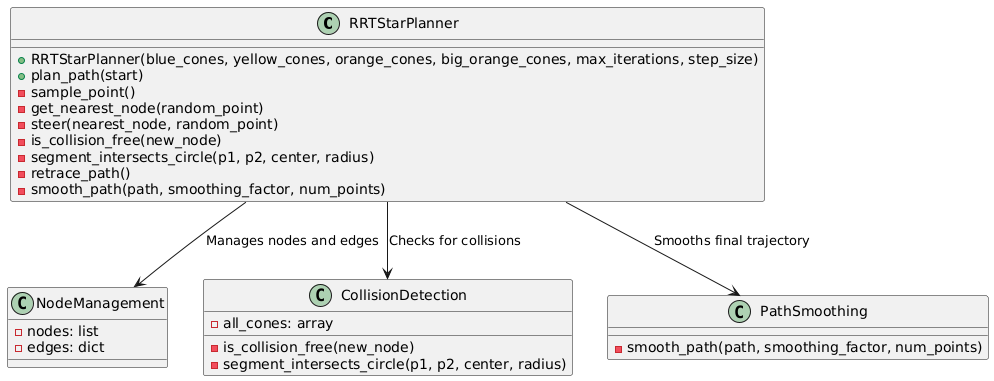
\includegraphics[width=\textwidth]{Images/rrt.png}
    \caption{RRT* Path Planning Structure}
    \label{fig:rrtstar_structure}
\end{figure}

RRT* was selected because of its capability to generate adaptive paths in dynamic
environments while ensuring path optimisation over iterations. The planner
comprises major modules which are node expansion, collision avoidance, and
final path smoothing.

\subsection{RRT vs. RRT*: Key Differences}

Though both RRT (Rapidly-exploring Random Tree) and RRT* (RRT Star)
belong to the same family of sampling-based path planning algorithms,
they serve different purposes when applied to real-world autonomous systems \cite{reference1, reference3}.
RRT is designed to quickly find any feasible path from a start to a goal state.
It is computationally efficient and particularly useful in high-dimensional configuration spaces.
It does not assure path optimality, sometimes leading to jagged or overly long routes.
On the other hand, RRT* incrementally optimises the path length and smoothness by continuously rewiring the tree during expansion \cite{reference4}.

In our autonomous car, optimality and continuity are not just desired; they are essential.
The OBRA car works in a limited and dynamic workspace set by cones that can vary in how close
they are to each other and even if they are there because of sensor limits. In such situations, just finding a safe path as RRT does, is not enough.
Paths must not only avoid obstacles but also minimise sudden steering changes but also minimise sudden
changes in a maneuver double delta at all times.
To improve lap times, the planner aims to produce smoother steering profiles and trajectories that 
adhere closely to the optimal racing line.

RRT* meets these requirements. By incrementally improving the path as new nodes come in, it makes
trajectories that are smoother and more centered. This cuts mechanical strain on the car's steering
system and raises overall stability, most especially in high-speed parts or tight turns. Also, the
capability of RRT* to change with local shifts in the environment makes it more strong for
real-time racing, where missing cones or sudden layout shifts may occur.

Although RRT* incurs a slightly higher computational cost due to its optimisation phase, 
we have some ways to tamp that down by carefully tuning parameters like step size
and maximum iterations. The end result is a planner that can work within the real-time
constraints of our onboard system and still come up with better paths than before. For
this reason, RRT* was chosen as the foundation
for our planner, offering a balance between flexibility, efficiency, and trajectory quality that
aligns with the specific demands of the OBRA car and the racing domain.

\subsection{Initial RRT* Planner: Centerline Trajectory}

To compare the RRT* planner with the Delaunay-based planner,
the first version of RRT* was made to track along a path biased toward the center of the track;
This decision was motivated by the behavior of the Delaunay planner, which inherently produces paths 
that pass through the midpoints of adjacent cones. Therefore, to center the implementation of RRT* 
enables a direct evaluation in terms of smoothness, adaptability, and precision under similar constraints.

To create this central bias, the picking function \texttt{sample\_point()} was built to make
random points with a liking for the shape center between blue and yellow cones.
This is done by finding the average position of cones on both sides of the
path and leading new random points toward that mean:

\begin{verbatim}
track_center_x = (np.mean(self.blue_cones[:, 0]) + 
np.mean(self.yellow_cones[:, 0])) / 2
track_center_y = (np.mean(self.blue_cones[:, 1]) + 
np.mean(self.yellow_cones[:, 1])) / 2
track_center = np.array([track_center_x, track_center_y])
...
random_point = 
random_point * (1 - bias_factor) + track_center * bias_factor

\end{verbatim}

A \texttt{bias\_factor} of 0.2  ensures that while points retain some randomness to enable
exploration, they are gently pulled towards the central path. Also, a slight outward
shift is applied to increase spacing from the cones and reduce the risk of near collisions:

\begin{verbatim}
shift_distance = 1.2
random_point += shift_distance * (random_point - track_center) / 
np.linalg.norm(random_point - track_center)
\end{verbatim}

Therefore, the resulting tree grows along the center of the corridor defined by the cones
such that it gives rise to paths which are smoother and better aligned with the properties of the Delaunay planner.
This set up is critical to extracting the specific advantages of RRT*, that it
can adapt to missing cones or sharper turns without any form of bias introduced by fundamentally different target trajectories.

Future versions of the planner, discussed in the next section, will explore more 
aggressive strategies focused on minimising lap time rather than maintaining central alignment.


\subsubsection*{Node Expansion and Distance Selection}

The RRT* planner expands nodes in the direction of randomly sampled 
points in front of the car to explore the space efficiently. The step size is set to \textbf{5 units} 
to balance coverage and computational efficiency:

\begin{verbatim}
def steer(self, nearest_node, random_point):
    """
    Generates a new node in the direction of `random_point`, 
    limited by `step_size`.
    """
    direction = (random_point - nearest_node) / 
    np.linalg.norm(random_point - nearest_node)
    new_node = nearest_node + direction * self.step_size
    return new_node
\end{verbatim}

Increasing the number of nodes improves path resolution as well but with
computational overhead. If too many nodes are generated per loop, 
the planner overloads the CPU, leading to a \textbf{delayed response} from the car. 
This makes the car react too late to try to follow the planned path, eventually causing it
to deviate off the track. An equilibrium was found
It turned out that \textbf{25 iterations} provide a good trade-off between accuracy and real-time performance.

\subsubsection*{Collision Detection and Safety Constraints}

To ensure the vehicle avoids obstacles, a collision-checking mechanism was implemented. 
Each new node is validated against the detected cones to ensure a \textbf{safe clearance distance} of at least \textbf{2.5 units}:

\begin{verbatim}
def is_collision_free(self, new_node):
    """
    Returns `True` if `new_node` does not collide with any cone.
    """
    safe_distance = 2.5  # Min clearance from cones
    distances = np.linalg.norm(self.all_cones - new_node, axis=1)
    return np.all(distances > safe_distance)
\end{verbatim}

By maintaining a safe distance from cones, the planner prevents situations where the vehicle may clip obstacles due to minor inaccuracies in perception.

\subsubsection*{Path Retracing and Smoothing}

Once a set of valid nodes has been generated, the planner reconstructs the path 
from the last node back to the start using a retracing mechanism:

\begin{verbatim}
def retrace_path(self):
    """
    Reconstructs the path from the last node to the start.
    """
    last_node = self.nodes[-1]
    path = [last_node]
    while tuple(path[-1]) in self.edges:
        path.append(self.edges[tuple(path[-1])])
    path.reverse()
    return np.array(path)
\end{verbatim}

To further refine the trajectory, a \textbf{spline-based smoothing algorithm} is applied. 
This ensures the path is continuous and minimises abrupt steering changes:

\begin{verbatim}
def smooth_path(self, path, smoothing_factor=0.5, num_points=50):
    """
    Uses spline interpolation to generate a smoother trajectory.
    """
    tck, u = splprep([path[:, 0], path[:, 1]], s=smoothing_factor, 
    k=min(3, len(path)-1))  
    x_smooth, y_smooth = splev(np.linspace(0, 1, num_points), tck)
    return np.vstack((x_smooth, y_smooth)).T
\end{verbatim}

Smoothing eliminates unnecessary oscillations in the path, 
reducing the load on the vehicle's steering system and improving driving stability.


\subsection{Final RRT* Planner: Fastest Trajectory}

Before all tests were carried out, this version of the RRT* planner, in theory, 
was thought to be the most optimal for the OBRA car. It was meant to give precedence 
to the shortest and most aggressive path along the track, rather than simply following 
the center line. While the first version of the RRT* favored a middle-line approach to 
give a clear contrast with the Delaunay planner, this iteration places more emphasis on agility, 
speed, and assertive maneuvering—key attributes in a competitive racing environment \cite{reference4}.

A major variation is in the sampling approach. Rather than choosing points that are
skewed towards the center of the track, as in the former case, this planner now selects
points which are more spread out along the driving axis (positive X-direction), thus
urging the vehicle to move forward rapidly while keeping lateral deviation to a minimum.
This is reflected in the following line within the \texttt{sample\_point()} method:


\begin{verbatim}
rand_x = np.random.uniform(5, 10)  # Prioritise forward sampling
rand_y = np.random.uniform(-3, 3)  # Allow lateral flexibility
random_point = np.array([car_x + rand_x, car_y + rand_y])
\end{verbatim}

To further enhance safety and maintain aggressive yet reliable driving, sampled points are rejected if they fall too close to any cone:

\begin{verbatim}
distances = np.linalg.norm(self.all_cones - random_point, axis=1)
if np.any(distances < 2.5):
    return self.sample_point()
\end{verbatim}

This ensures that the trajectory not only favors speed but also remains within safe operational margins.

Also, this version uses an alignment-weighted nearest node search that
emphasises growth in the positive direction (X-axis), strengthening the planner’s
preference for the racing line and making sure there are no backward or wasteful
excursions.

\begin{verbatim}
goal_direction = np.array([1, 0])  # Favors forward motion
\end{verbatim}

Compared to the initial centerline-focused RRT*, this implementation results in more
aggressive paths that cut closer to the apex of turns and reduce total lap distance,
while still respecting safety constraints. It is therefore better aligned with the real-world
demands of autonomous racing, where maximising performance per lap is more important than symmetrical navigation.

his final RRT* planner establishes a strong foundation for real-world deployment in the real vehicle, 
offering a robust balance between real-time feasibility, adaptability, and competitive performance.

\subsection{Final Considerations}

Throughout this project, three distinct path planners were developed and four were evaluated to explore the trade-offs between 
stability, adaptability, and performance in autonomous racing: the initial unoptimised Delaunay planner, 
the improved Delaunay version, a centerline-biased RRT* planner, and the final optimised RRT* for fastest trajectory.

The first \textbf{Delaunay} solution was the one the car was already using. It was functional but lacked flexibility
to manage dynamic track variations; it used a fixed triangulation logic between cones, often
generating stable but suboptimal paths \cite{reference6}. Consequent weaknesses were exposed with unstable
configurations, that is, with missing or misplaced cones, and with sharper turns, where greater
dynamic trajectory adaptation was required.

The \textbf{Optimised Delaunay} version made some steps toward this, by refining the triangulation logic,
improving the selection of midpoints and parameters to make the output path more consistent.
It still suffered structural rigidity since its connectivity depended on the presence and layout of
detected cones. It offered much better stability than the original version, but its adaptability and
response time to sudden track changes remained limited.

To overcome these constraints, the family of RRT* planners was introduced. The first implementation of \textbf{Centralised RRT*} was 
intentionally biased toward the centreline to mirror the typical behavior of the Delaunay planner.
This allowed a fair comparison in terms of precision, smoothness, and structural differences \cite{reference3}.

The final and theoretically most performant version is the \textbf{Optimised RRT*} planner targeting the fastest possible trajectory.
No longer does it follow a geometric centerline like its predecessors, but it actively searches for paths that minimise 
total driving distance and improve lap time. It generates more aggressive and efficient routes through strategic forward sampling, 
directionally weighted node expansion, and active cone avoidance \cite{reference4}.
It is expected that the final RRT* planner will significantly outperform 
the others in dynamic conditions, especially on sharp turns and incomplete cone layouts. 
Its adaptive nature and path optimisation capabilities make it the most promising solution for real-world autonomous racing.

\section{Version Management}

Version control has a great part in the building of this project. It helps run collaboration,
control code, keep it in order and track changes as well. So, we use Git and
have GitLab where the OBRA team's shared workspace is kept. Here, GitLab acts as the main repository
that keeps all project files, code versions, and data from previous years \cite{reference18}.

At the beginning of the project, the entire existing workspace was cloned from GitLab, 
providing access to all prior developments, including path-planning algorithms and other essential 
components used by the team in past seasons. This initial setup allowed us to build on a strong foundation 
while ensuring compatibility with the existing autonomous system.

Throughout the development process, every modification and enhancement to the path planners 
has been systematically handled using branches within our GitLab repository. Each time a new version 
of a path planning algorithm was implemented—whether adjustments to the Delaunay planner or the creation of the RRT* algorithm—an exclusive branch was opened. 
This branching strategy enabled parallel development and evaluation of diverse versions while maintaining the stability of the main codebase \cite{reference18}.

Commits are made in an organised and regularly updated repository, from which every iteration and 
refinement is documented. This has been key in ensuring traceability and rollback capabilities when needed, 
as well as enabling effective collaboration. With GitLab’s integrated features, we set up a structured 
development flow, making code reviews, bug tracking, and continuous integration more manageable.

In addition to code management, we use Notion to coordinate team tasks and maintain an Agile workflow. 
Notion enables us to assign responsibilities, track progress, and ensure development efforts remain aligned 
with project goals. Furthermore, all generated data, including test results, simulation outputs, and performance 
evaluations, are stored in Google Drive. This provides a centralised location for data accessibility, allowing for 
efficient documentation and analysis of algorithm performance over time.


\newpage

\chapter{Testing and Evaluation}

This chapter gives the evaluation methodology and results of four path planning algorithms: Original Delaunay, 
Optimised Delaunay, Central RRT*, and Optimised RRT*. All planners undergo testing in controlled simulations having identical 
dynamics, with performance evaluated in terms of lap time and average speed as well as trajectory smoothness using metrics relevant to autonomous racing.

\section{Results and Testing}

The evaluation of the four planners—Original Delaunay, Optimised Delaunay, Central RRT*, and Optimised RRT*—
was held in a unified simulation environment to assure consistency and fairness across tests.
The setup was done using the Unity game engine, where a closed-loop racetrack, designed to simulate
realistic driving conditions, was made custom for this vocation \cite{reference17}.
The virtual track served as the benchmark environment for assessing the path planning capabilities of each algorithm,
as illustrated in Figure~\ref{fig:simulator}.

\begin{figure}[H]
    \centering
    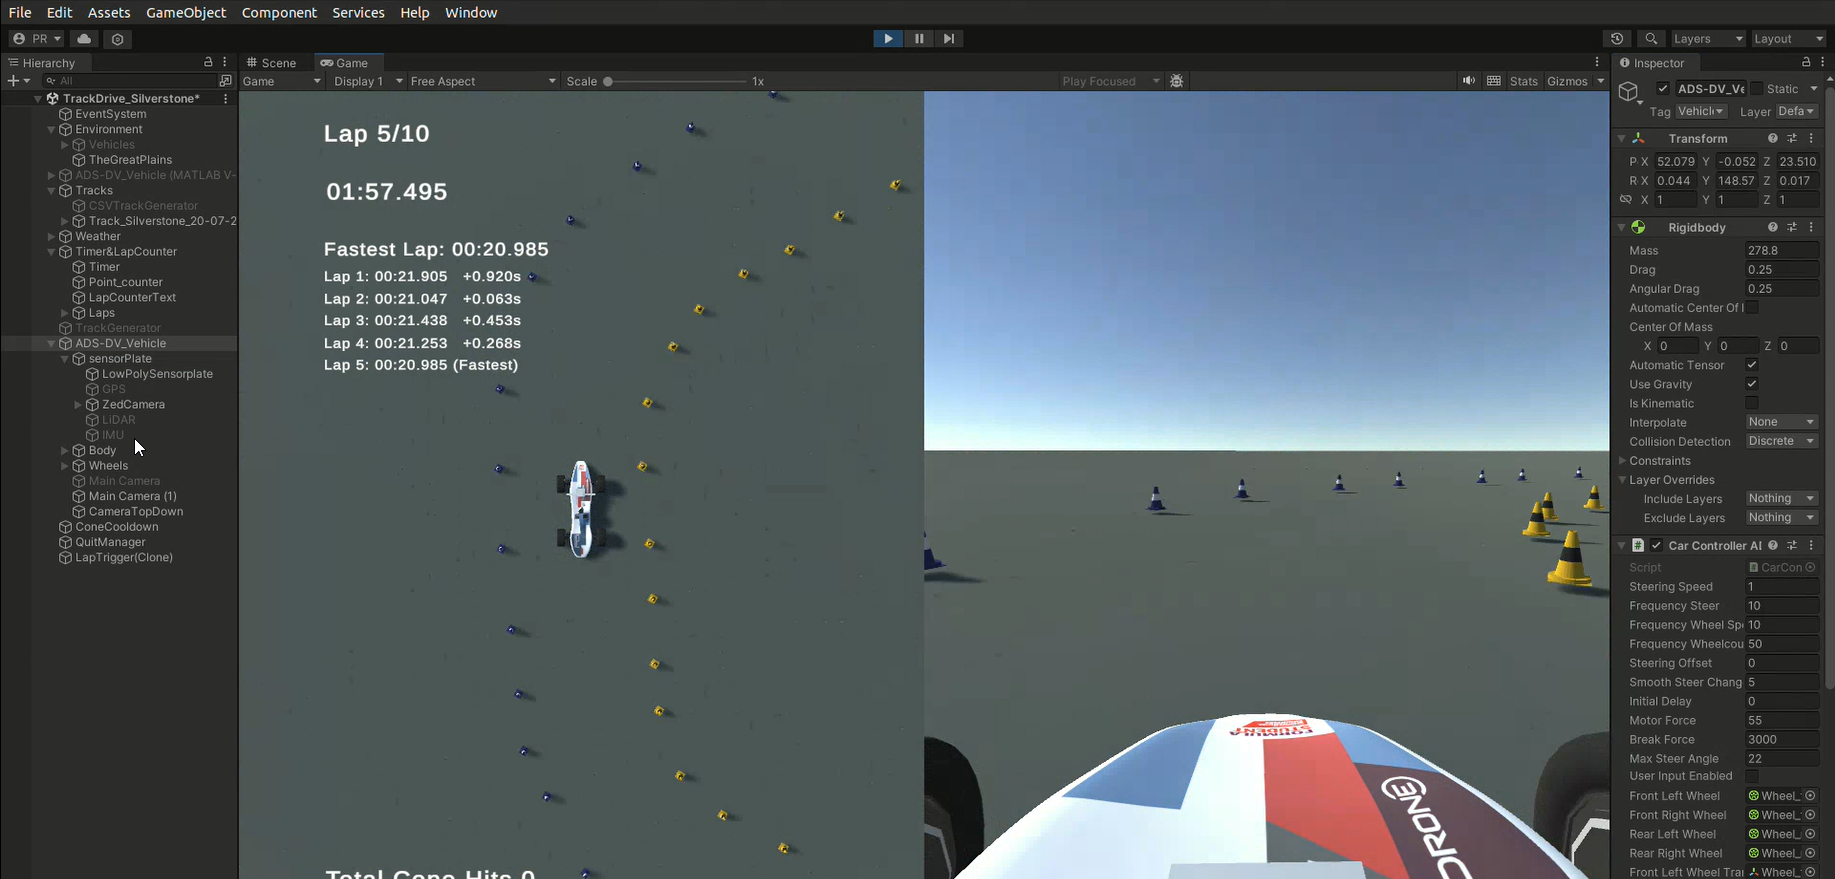
\includegraphics[width=0.95\textwidth]{Images/simulator.png}
    \caption{Simulation environment developed in Unity for planner evaluation}
    \label{fig:simulator}
\end{figure}

To monitor and validate the system behavior, \texttt{Foxglove Studio} was employed as the 
main visualisation tool. It allowed real-time inspection of topics published during the simulation, 
such as \texttt{/planned\_path}, \texttt{/vehicle\_pose}, and \texttt{/smooth\_trajectory}, as illustrated in Figure~\ref{fig:foxglove}.

\begin{figure}[H]
    \centering
    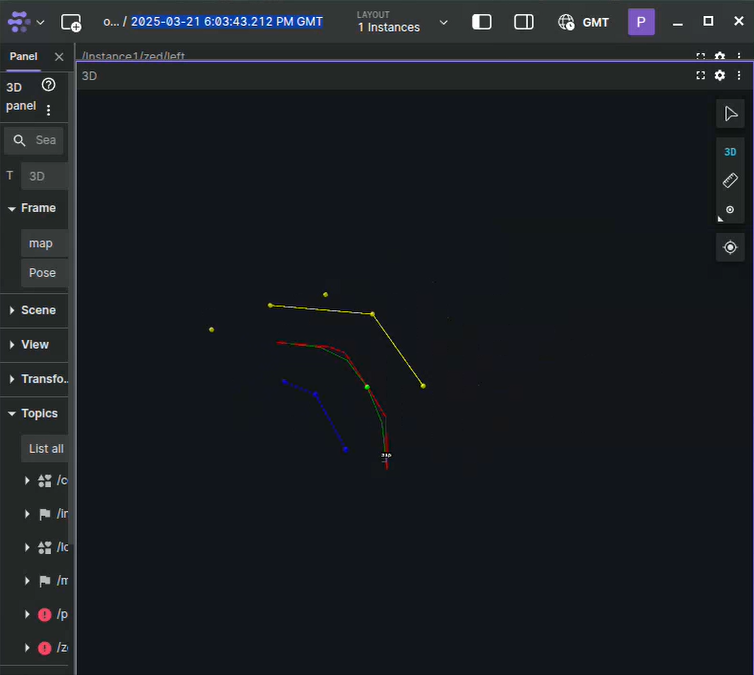
\includegraphics[width=0.95\textwidth]{Images/foxglove.png}
    \caption{Foxglove environment developed for trajectory evaluation}
    \label{fig:foxglove}
\end{figure}

To guarantee that all planners were being tested under identical physical conditions,
we applied a constant engine force value to the vehicle in Unity for every test case.
The parameter controls the forward propulsion of the car, and keeping it fixed would
guarantee that all planners have the same opportunity to accelerate and complete each lap.
As a result,
lap times should be within the same range across planners and any observed variations in 
execution time can be attributed solely to the performance and efficiency of the path planning algorithm itself.

This standardised setup ensured that all planners operated under identical conditions; 
same track layout, vehicle dynamics, environmental parameters, and simulation duration.

\subsection{Results and Testing, Test 1}
The initial test scenario consisted of a single simulation session per planner, 
in which each executed three complete laps around a closed-loop racetrack. 

While it ran,
the positions (X, Y, Z) coordinates and timelaps were captured in Unity and then, in CSV format, exported right after the simulation.
As a result, the CSV files had high resolution in them
space and time data, which enabled accurate analysis for computing performance metrics 
such as execution time, path length, and speed profiles.
The planners evaluated in this stage were:

\begin{itemize}
  \item Original Delaunay
  \item Optimised Delaunay
  \item Central RRT*
  \item Optimised RRT*
\end{itemize}

The track used for this test was a simplified representation of a real-life course, based on the "Silverstone FS-UK 2024" circuit. 
he experiment was conducted in a fully controlled environment, free from dynamic parts like moving obstacles, 
in order to enable a direct comparison of the planners’ trajectory generation capabilities. 
A constant propulsion force of 45 Unity units, corresponding approximately to 31.6 km/h, was applied
for the motor force.

To evaluate the execution time taken by each path planner, we measured the time the planner took to complete 
each of the three laps during the simulation. The table below gives the lap times recorded for the four tested planners.

\begin{table}[H]
    \centering
    \begin{tabular}{lccc|c}
    \toprule
    \textbf{Planner} & \textbf{Lap 1 (s)} & \textbf{Lap 2 (s)} & \textbf{Lap 3 (s)} & \textbf{Average (s)} \\
    \midrule
    Central RRT* & 39.115 & 38.197 & \textbf{37.748} & 38.353 \\
    Original Delaunay & 39.202 & 37.777 & \textbf{37.682} & 38.220 \\
    Optimised Delaunay & 39.162 & \textbf{37.436} & 37.584 & \textbf{38.061} \\
    Optimised RRT* & 39.420 & 37.630 & \textbf{37.093} & \textbf{38.048} \\
    \bottomrule
    \end{tabular}
    \caption{Lap times and averages for each planner. Best lap per planner and top two average times are highlighted in bold.}
    \label{tab:lap-times}
    \end{table}
    
Figure~\ref{fig:lap-times-plot} gives a visual comparison of the lap times.
\begin{figure}[H]
\centering
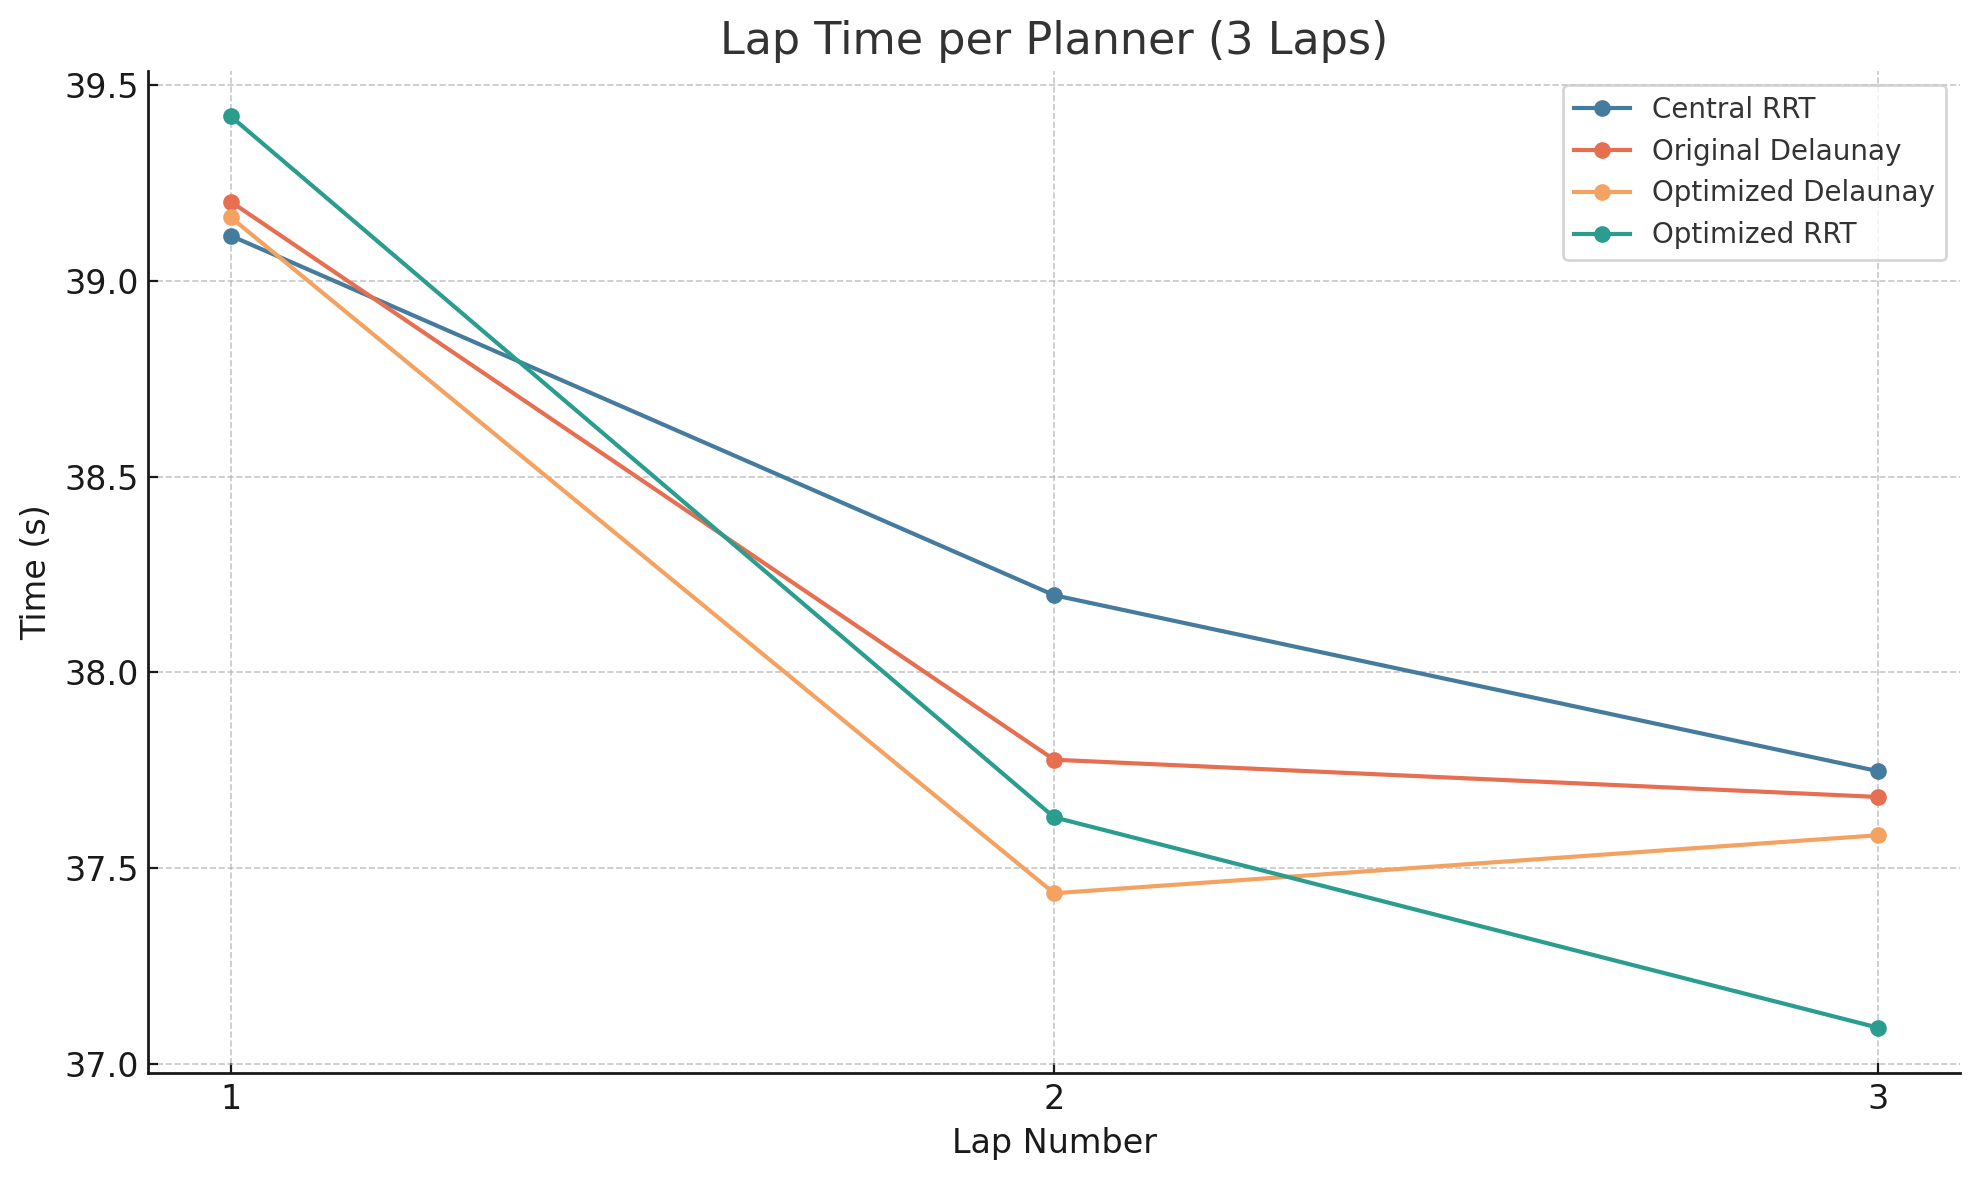
\includegraphics[width=0.9\textwidth]{Images/lap_time_table_plot_colored.png}
\caption{Comparison of lap times across planners. Delaunay variants are shown in warm tones; RRT variants in cool tones.}
\label{fig:lap-times-plot}
\end{figure}

To evaluate the quality of the planned trajectories, 
two primary metrics were considered: \textbf{average speed} and \textbf{path smoothness}. 
These metrics are crucial in autonomous racing, where both time efficiency and stability at 
high speeds are essential.

All planners were tested using the same simulated conditions and speed controller, 
configured to maintain a consistent target velocity of approximately 31 km/h (8.6 m/s). 
\begin{table}[H]
\centering
\begin{tabular}{|l|c|}
\hline
\textbf{Planner} & \textbf{Average Speed (m/s)} \\
\hline
Delaunay & 4.29 \\
Delaunay Optimised & 4.32 \\
Central RRT* & 4.31 \\
RRT* Optimised & 4.30 \\
\hline
\end{tabular}
\caption{Average speed comparison across path planners}
\label{averagespeed}
\end{table}

Smoothness was calculated by averaging the absolute angular variance between successive path segments.

\begin{table}[H]
    \centering
    \begin{tabular}{|l|c|}
    \hline
    \textbf{Planner} & \textbf{Average Smoothness (rad)} \\
    \hline
    Delaunay & 0.8405 \\
    Delaunay Optimised & 0.8226 \\
    RRT & 0.8043 \\
    RRT Optimised & 0.7885 \\
    \hline
    \end{tabular}
    \caption{Smoothness comparison of the generated paths}
    \label{smoothness}
    \end{table}


\begin{table}[H]
    \centering
    \begin{tabular}{|l|c|c|c|}
    \hline 
    \textbf{Planner} & \textbf{Avg. Lap Time (s)} & \textbf{Avg. Speed (m/s)} & \textbf{Smoothness (rad)} \\
    \hline
    Original Delaunay & 38.22 & 4.29 & 0.8405 \\
    Optimised Delaunay & 38.06 & 4.32 & 0.8226 \\
    Central RRT* & 38.35 & 4.31 & 0.8043 \\
    Optimised RRT* & 38.05 & 4.30 & 0.7885 \\
    \hline
    \end{tabular}
    \caption{Aggregate comparison of all planners.}
    \label{tab:summary}
    \end{table}
        
    
\subsection{Results and Testing, Test 2}

Based on the results of the initial tests, a second more extended simulation will be set up to analyse long-term
performance and consistency. A total of 20 consecutive laps were executed and is performed only for the two top
performers from the first round. The objective is to measure stability
across multiple laps as well as to identify variations in the lap time and assess the repeatability
the path planning logic during a longer session. The motor force for this test will be; \texttt{55 units} (39,9 km/h)

Based on the previous analysis, the two best-performing planners in terms of average 
speed and smoothness were the \textbf{Delaunay Optimised} and \textbf{RRT* Optimised} versions. 
Both demonstrated competitive performance and path quality, making them suitable candidates for 
further testing.

The next phase of the evaluation involves a larger-scale simulation consisting of \textbf{20 consecutive laps} 
using again a  a real world racing circuit. Specifically, the test will take place on the 
track used during the FS-UK 2022 competition. The map of the circuit is shown in Figure~\ref{fig:track}.

The following graphs show our findings in terms of lap consistency, laptime distribution, and trajectory behavior.

\begin{figure}[H]
    \centering
    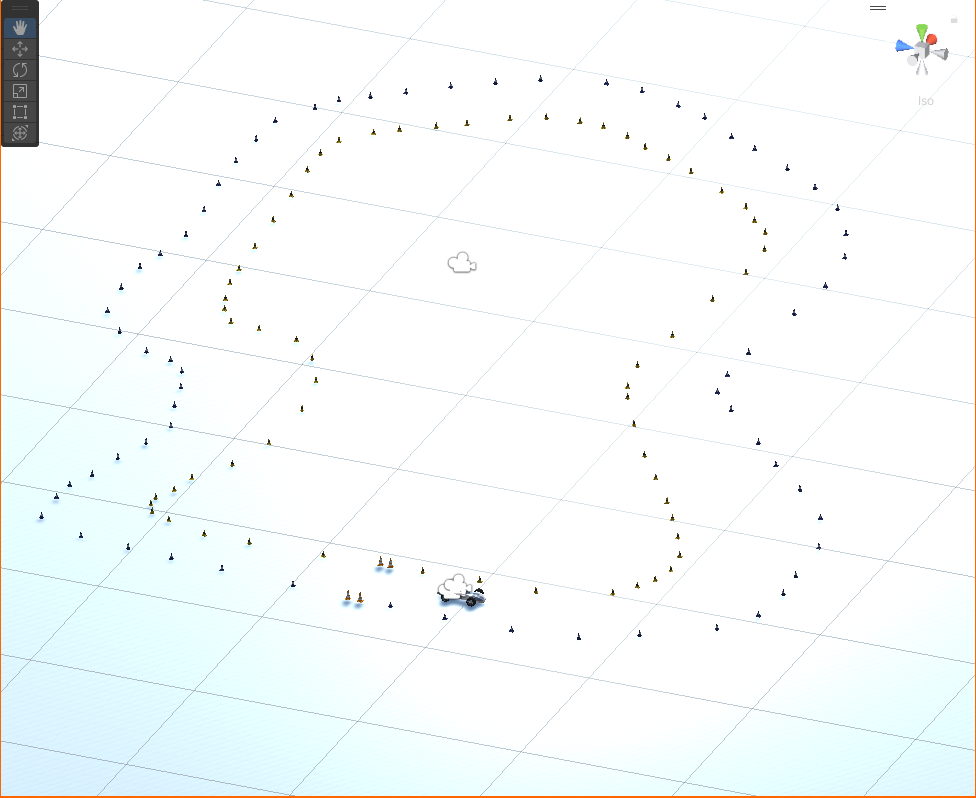
\includegraphics[width=0.90\textwidth]{Images/Track.png}
    \caption{Circuit used for extended testing — FSUK 2022 layout}
    \label{fig:track}
\end{figure}

This setup will allow a rigorous assessment of consistency, stability, 
and overall suitability of the planners for real-world deployment. 
The outcome will guide the final recommendation for planner integration 
into the OBRA autonomous vehicle system.

Figure~\ref{fig:overlay} shows the lap times for each of the 20 laps.
\begin{figure}[H]
    \centering
    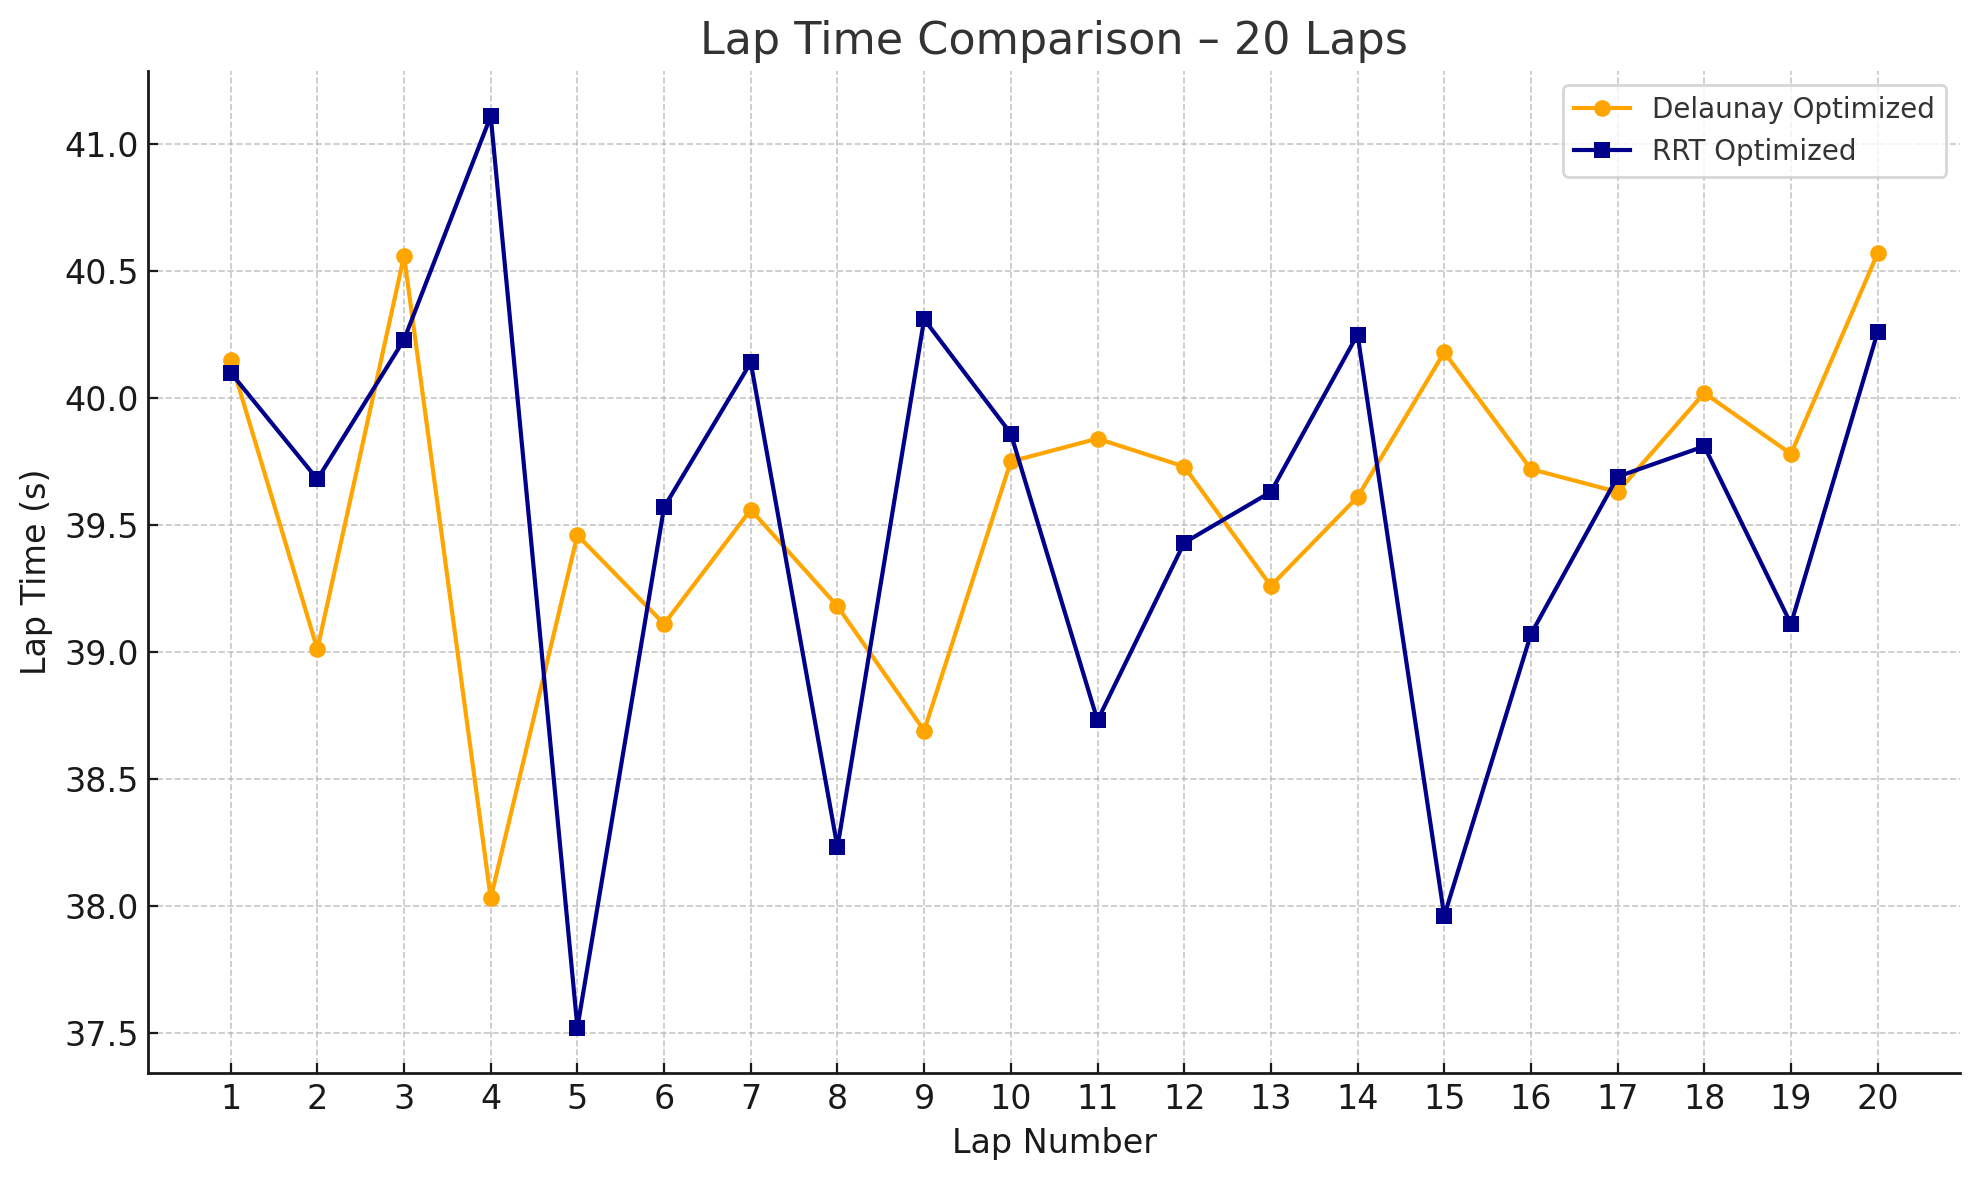
\includegraphics[width=0.9\linewidth]{Images/RRTvsDELAUNAY.png}
    \caption{Overlay of RRT* and Delaunay trajectories across 20 laps.}
    \label{fig:overlay}
\end{figure}

Figure~\ref{fig:distribution} illustrates the distribution of lap times for both planners. 
\begin{figure}[H]
    \centering
    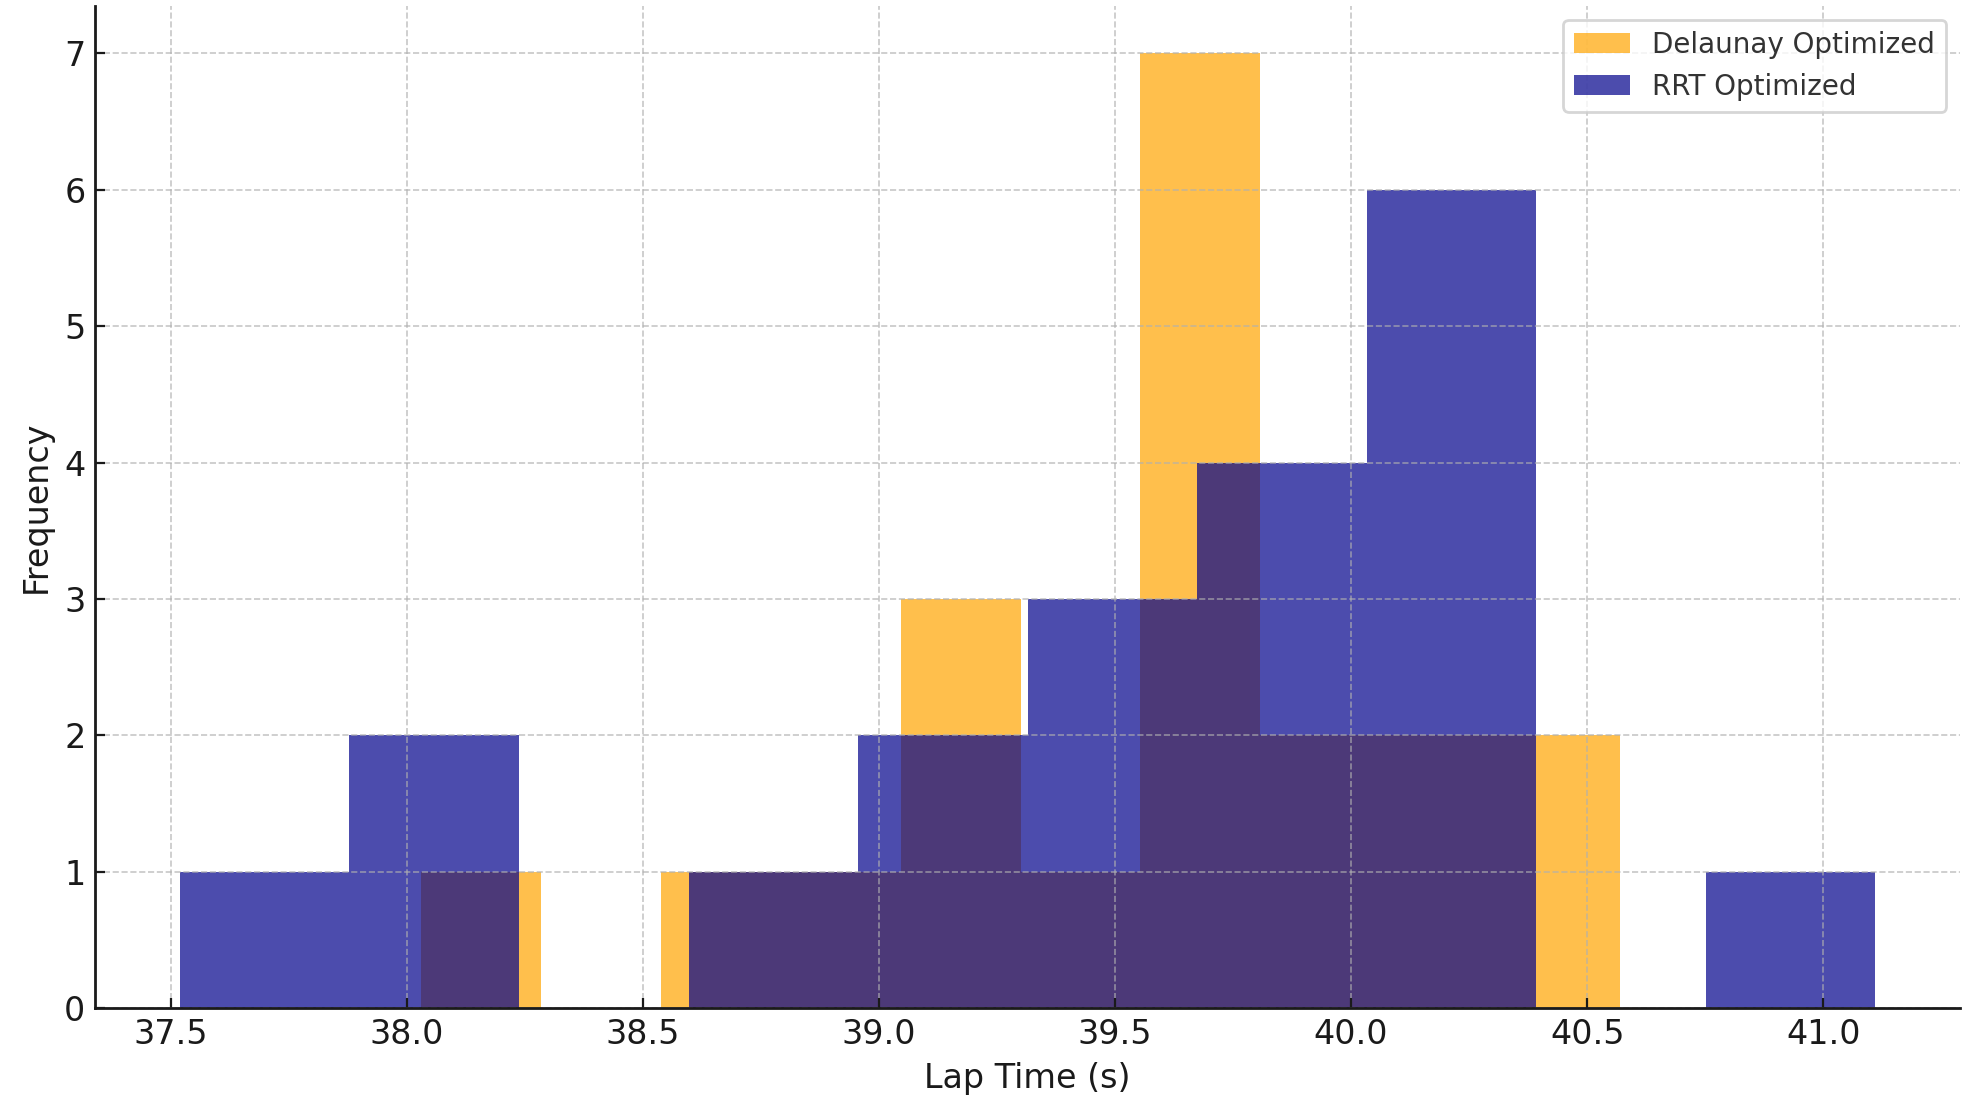
\includegraphics[width=0.9\linewidth]{Images/Laptimedistribution.png}
    \caption{Lap time comparison between Delaunay Optimised and RRT* Optimised.}
    \label{fig:distribution}
\end{figure}

At last, Figure~\ref{fig:laptime} compares the boxplot between the Delaunay Optimised and RRT* Optimised planners. 
\begin{figure}[H]
    \centering
    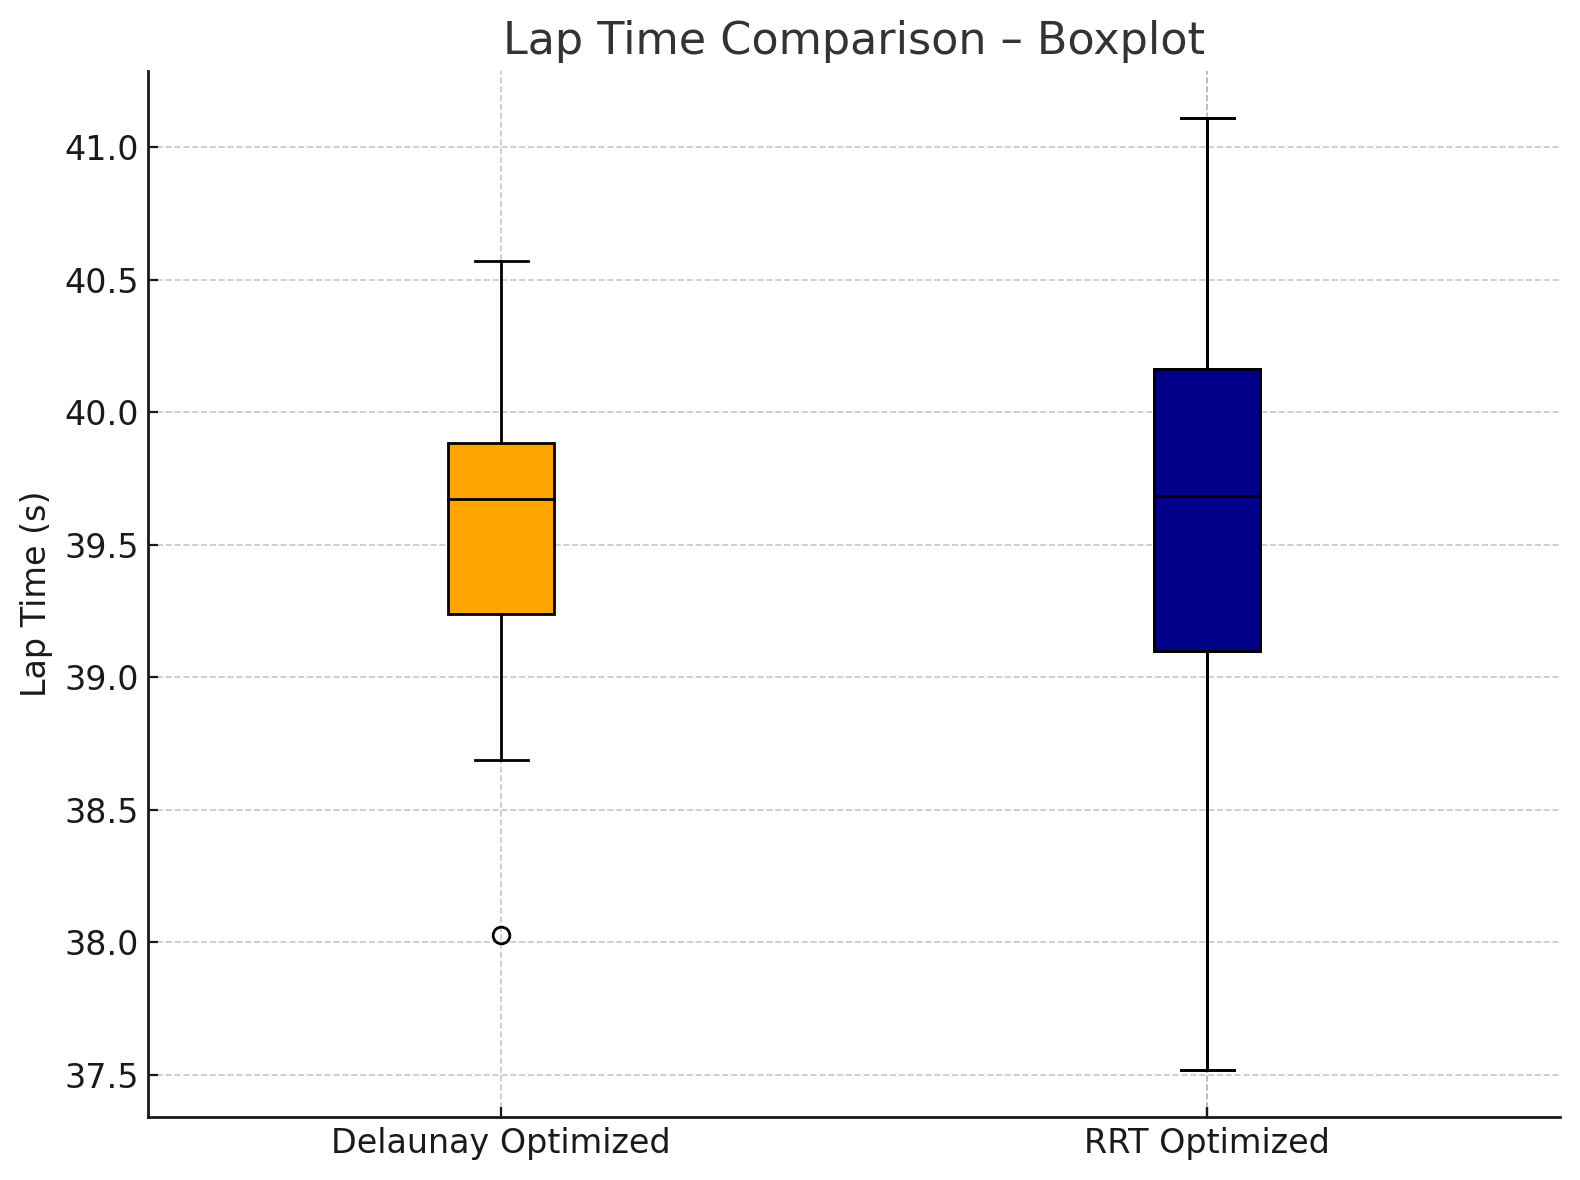
\includegraphics[width=0.95\linewidth]{Images/Laptimecomparaison.png}
    \caption{Lap time distribution histogram comparing, average mean, standard deviation, and outliers.}
    \label{fig:laptime}
\end{figure}

\section{Discussion}
\subsection{Discussion, Test 1}
\subsubsection*{Lap Time Comparison}

Figure~\ref{fig:lap-times-plot} gives a visual comparison of the lap times, allowing us to analyse the
consistency and evolution of performance over laps. All planners show similar total times
since the same propulsion force is applied during simulation, yet minor variations in trajectory
length and smoothness, born by the different planning strategies, account for the disparities in
lap times \cite{reference6}.

\subsubsection*{Average Speed}

Due to the path curvature and minor variations in the generated trajectories, the resulting 
average speeds remain very close across all methods, as shown in \ref{averagespeed}. This ensures a fair comparison focused on the planners' 
structural differences rather than speed discrepancies.

\subsubsection*{Path Smoothness}

The metric reflects in \ref{smoothness}, trajectory continuity and curvature, with lower values indicating smoother paths and thus
better suitability for high-speed navigation. As expected, the optimised versions of both planners produced
smoother trajectories, being the RRT* Optimised considerably better, with the lowest average angular change.


\subsection{Discussion, Test 2}
To understand the differences in performance between the optimised Delaunay planner and the optimised RRT*, 
several visual comparisons were then created after the 20-lap test on the FSUK 2022 track. 

\subsubsection*{Lap time comparison}
Figure~\ref{fig:overlay} shows the lap times for each of the 20 laps. Both planners exhibit similar average speeds, 
consistent with the fixed motor speed of approximately 31 km/h across all tests. However, the RRT* planner 
displays more volatility in its lap times. While the
Delaunay planner shows steady performance, with most laps’ times clustering around the mean, the RRT* planner
achieves several laps of much faster times with some interspersed
with others that are notably slower. This 
implies that due to its randomised tree exploration
nature, occasionally detects highly efficient routes
or "lucky branches" as well but also suffers from
suboptimal paths in some iterations.
This is exactly the theoretical characteristic of RRT*. Since its random sampling allows for
fast pathfinding and frequently checks out new routes to dynamically find them,
this could consequently lead to high performance in some laps
but at the same time, a much lower degree of consistency.

\subsubsection*{Lap time distribution}
Figure~\ref{fig:distribution} illustrates the distribution of lap times for both planners. 
The Delaunay histogram follows a narrower and more symmetric shape, indicating greater consistency and a lower 
standard deviation. The RRT* distribution is wider and less predictable, with a few laps reaching exceptional 
performance (outliers below 38,5 s), and others exceeding 40s. Quantitatively, the standard deviation for RRT* was approximately 
\textbf{0.73 seconds}, while Delaunay's was lower, at around \textbf{0.43 seconds}. This validates that while RRT* can be faster, 
it also introduces more performance uncertainty.

\subsubsection*{Lap time Overlay}
At last, Figure~\ref{fig:laptime} compares the boxplot between the Delaunay Optimised and RRT* Optimised planners. 
Delaunay exhibits a tighter interquartile range with most of the lap times concentrated between approximately 39.2 and 40.0 seconds, 
with one outlier just under 38.5 seconds. RRT* exhibits a spread where the lap times are below 37.6 seconds and over 41 seconds. 
Although the median lap time for the latter is slightly better, the larger variability demonstrates that occasional high-speed laps come with 
a trade-off of reduced consistency.

\subsubsection*{Code Efficiency and Optimisation Metrics}

To complement the performance analysis of both planners, it is also important to evaluate their codebase and 
implementation characteristics, focusing on modularity, execution efficiency, and potential for scalability within the OBRA system.

From a structural standpoint, both the Delaunay and RRT* planners follow the same modular architecture illustrated earlier in 
Figure~\ref{fig:path_planning_structure}. 

In terms of code size, the Delaunay optimised planner comprises approximately \textbf{250 lines}, 
while the RRT* implementation consists of around \textbf{200 lines}. 
This similarity reflects a shared emphasis on clarity and modular design, with no significant difference in terms of overall complexity or readability. 

However, regarding runtime efficiency, some differences begin to emerge. The Delaunay planner demonstrates lower 
CPU usage under our current configuration. In contrast, the RRT* implementation, using parameters such as 25 nodes 
every 5 meters, incurs higher computational costs. This is expected given the sampling-based nature of RRT*, which involves 
iterative growth and optimisation of a tree structure \cite{reference3}.

\section{Issues Encountered}

Throughout the development and evaluation process, several challenges that affect the internal capabilities of the planners
or the external conditions under which they operate were identified.
These shall be classified into \textit{limitations}, being inherent aspects of the current implementations or testing scope, and
\textit{constraints}, the conditions provided by the execution environment or simulation setup.
Here's a table that sums up the main points from each category.

\begin{table}[H]
    \centering
    \begin{tabular}{|p{6cm}|p{6cm}|}
    \hline
    \textbf{Limitations} & \textbf{Constraints} \\
    \hline
    RRT* is in early-stage development & High CPU usage and hardware dependence \\
    \hline
    Delaunay planner is more mature and integrated & Processing lag can cause vehicle deviation \\
    \hline
    Testing limited to simulated environments & Constant motor force limits dynamic behaviour \\
    \hline
    No hyperparameter tuning performed & Unity lacks physical realism for deployment evaluation \\
    \hline
    \end{tabular}
    \caption{Summary list of identified limitations and constraints.}
    \label{tab:limitations_constraints_summary}
\end{table}

\subsection{Limitations}

From a software maturity perspective, the Delaunay planner has reached a more stable and adapted state. 
It is currently well-aligned with the OBRA car’s software and hardware stack and has undergone multiple cycles 
of refinement and tuning. On the other hand, the RRT* planner is still in an early stage of development.
This version was implemented from scratch during the current academic year and is undergoing its first rounds of validation.
Despite this, it has already achieved performance metrics that in some cases rival and even surpass those of the Delaunay planner. 
This is a promising sign, suggesting that with continued refinement and tuning, the RRT* algorithm has strong potential to outperform its counterpart in future iterations.

The present analysis has been done only in simulated settings. Actual testing on 
the OBRA car is still to happen, which limits the evaluation of the planners' robustness under unpredictable physical 
conditions like terrain vibration, sensor noise, or mechanical drift.

The performance of both planners was measured using default parameters or manual parameters. No systematic hyperparameter 
search was done, which might have unlocked further performance, especially for RRT*.

\subsection{Constraints}

The computational cost of the RRT* algorithm scales with the number of nodes and trajectories to be computed; this makes 
it highly hardware-dependent \cite{reference3}. On simple consumer-type computers, the algorithm is very greedy in terms of CPU cycles, often saturating it completely. 
This high processing overhead introduces perceptible lag in trajectory generation, which can slowly veer the car away from the ideal path.
As a result, the vehicle may deviate from the racing line or even leave the track, compromising both stability and overall performance.

A constant motor force was applied throughout all simulations. This made for an apples-to-apples 
comparison but at the same time, it shackled the planners from being able to modulate speed dynamically for complex trajectories.

The Unity environment is realistic, but it does not simulate physical effects such as tire slip, vibration feedback, 
or fine-grain terrain interaction. These limitations reduce the fidelity of the evaluation when comparing to real-world deployment \cite{reference17}.


\newpage

\chapter{Professionalism}
\section{Project Management}

The project was developed following a structured and professional flow based on the Agile style. 
Tasks were organised into iterations which reflected real-world software engineering practices, adaptive 
planning, early validation, and continuous improvement. Weekly supervisor meetings were set to be held early 
in the project wherein progress, discoveries and challenges were shared. 
Followed by questioning, clarification, and alignment on technical understanding. These meetings helped to keep the work on track, 
making it meaningful and academically sharp, and giving timely feedback and redirection when needed. Version control practices were applied 
all through the project. GitLab served as the main repository for source code and experimental results in line with industry-standard version control conventions.
Additionally, a private GitHub repository was maintained for general documentation and backup of supplementary files.

The complete workflow, structured into iterative development sprints, is shown in Figure~\ref{fig:agile_gantt}, which illustrates all 
key phases and their overlap across the project timeline. Each iteration addressed a different stage of the system's life cycle, 
from research and implementation to testing, validation, and integration. This approach allowed the project to remain flexible and 
reactive to technical challenges while maintaining clear deliverables and deadlines throughout the academic year.

\begin{figure}[H]
    \centering
    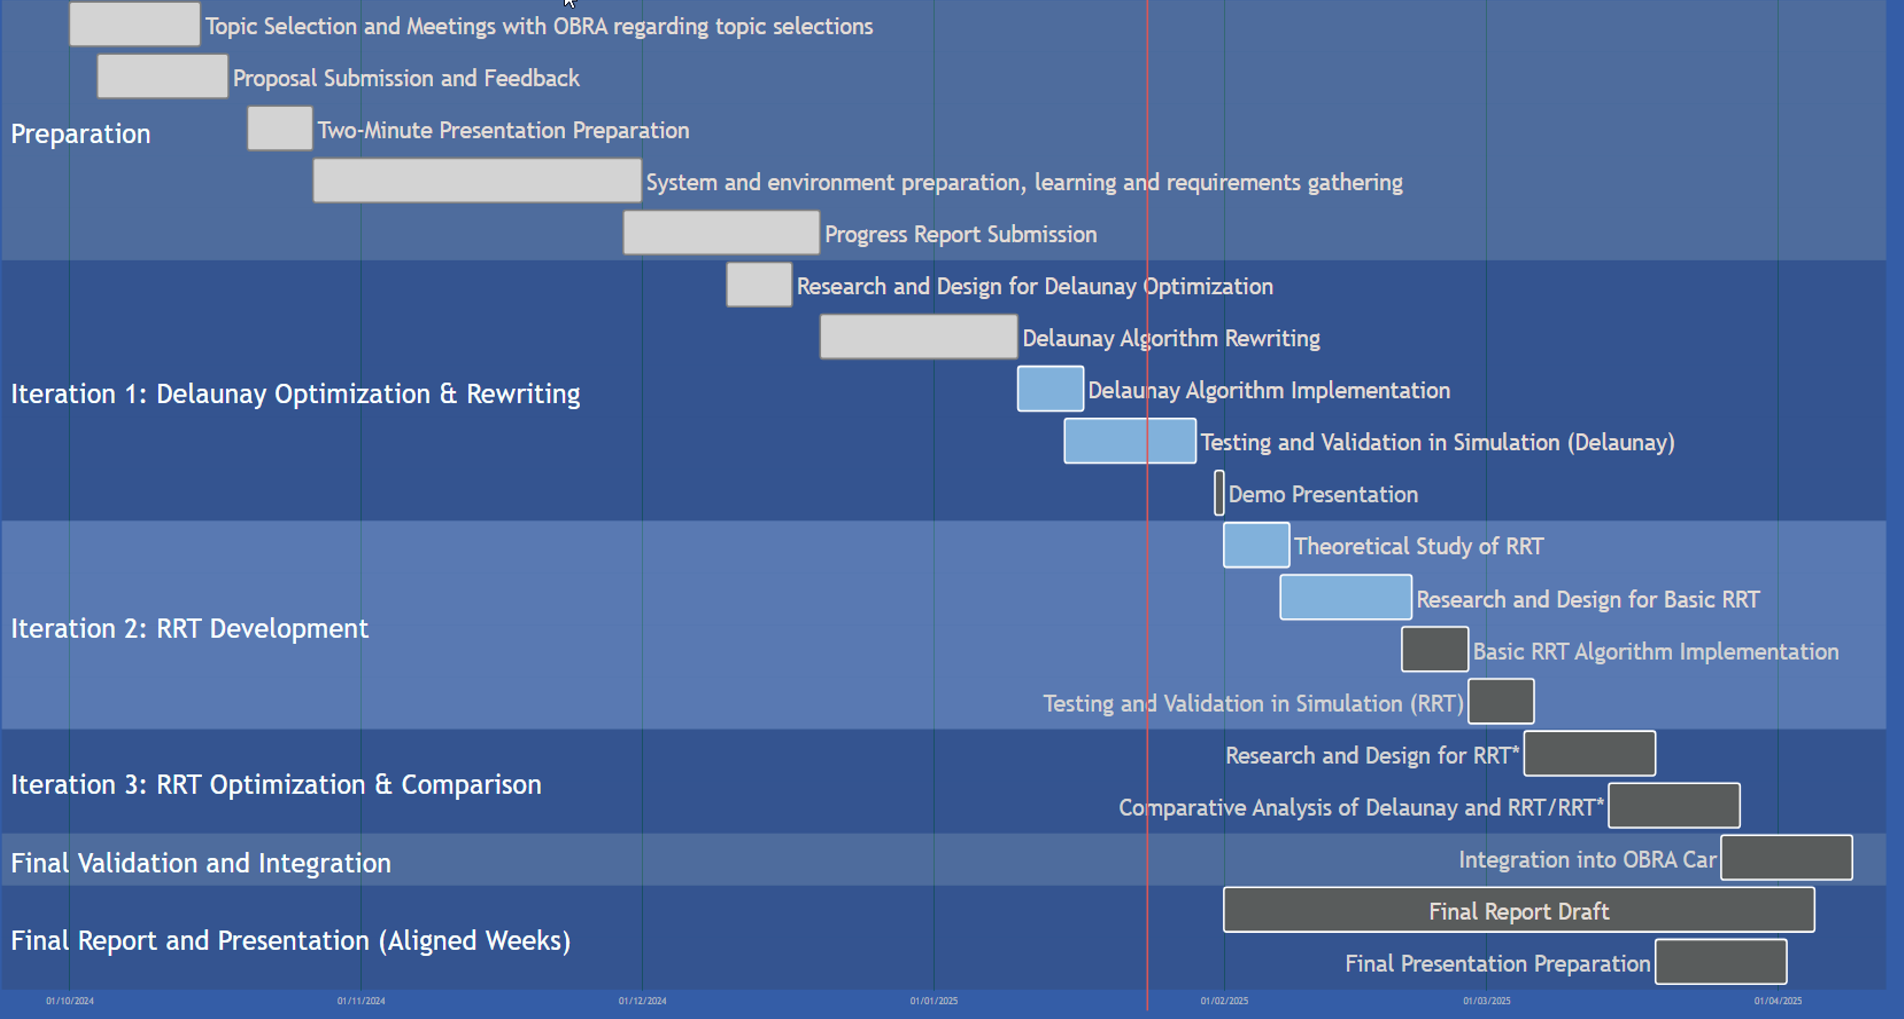
\includegraphics[width=1\textwidth]{Images/gant.png}
    \caption{Complete Project Timeline – Agile Workflow}
    \label{fig:agile_gantt}
\end{figure}

\section{Risk Analysis}
The project met risks in its inception, all of which were managed to minimise their impacts.
Delays have been a challenge in getting the RRT* algorithm into the system. The
refinement and rework of the Delaunay Path Planner became tenuous, causing the timeline for RRT* development to shift. 
This was mitigated by prioritising the completion of Delaunay optimisation and using 
Agile methodology to reallocate resources flexibly. The iterative nature of Agile has 
allowed for overlapping tasks, ensuring that progress on other deliverables continues 
without interruption.

Another risk involved the integration challenges for Unity and ROS2. Making algorithms
compatible with simulation tools involved more debugging and adjustment than
expected. To handle this, testing was done step-by-step in Unity to identify
problems early, and additional research on ROS2 compatibility was integrated into the development process.

Looking into the future, there are risks that must be mitigated.
One is the challenge of effectively comparing algorithm performance. To address this,
clear metrics like computational speed, route quality, and adaptability have been
defined. These now guide testing and analysis. Another risk is related to real-world
implementations. While simulations in Unity provide a controlled environment,
deploying in physical settings involves greater unpredictability.

There is also a risk of time constraints as deadlines approach. Regular progress 
evaluations and adherence to the Gantt chart will ensure the project remains on track.

\section{Professionalism}
This work holds major legal, ethical, and social considerations. Autonomous
car algorithms, can have potential real-world
applications in sectors like transportation and logistics, raising safety,
accountability, and access equity questions. This project will ensure
that by aligning codes of conduct, like those from BCS (British Computer
Society) and ACM (Association for Computing Machinery),  the project
compliance with professional codes of conduct for work and accountability.
Equity, Diversity, and Inclusion (EDI) has been factored in during the design.
The plan serves inclusivity by making certain the algorithms can apply to many
different situations and are available to all staff. Reports are circulated outside
the group to enforce cooperation, irrespective of where they come from, or how
skilled they may be.
IP becomes another key consideration. All code and results get stored in private
repositories for secure management and crediting to the OBRA team.
Proper version control practices using GitHub can add another layer in protecting the
integrity of the project at the same time maintaining transparency.
By addressing these risks and professional considerations, the project technically
attains the goals set for it while also ensuring that the outputs align with the prescribed ethical and legal standards.
making it relevant and useful for the real-world autonomous systems.
\newpage

\chapter{Conclusion and Future Work}

This project developed and evaluated four path planning algorithms—Optimised Delaunay, 
Central RRT*, and Optimised RRT*—alongside an existing Original Delaunay planner. 
All four planners were compared in every detail that could be thought of within the limits of a 
simulation environment in terms of lap time, average speed, and path smoothness. Results highlight 
variation in terms of consistency, computational cost, and overall trajectory quality with Optimised 
RRT* which shows much promise but also higher variability due to its sampling-based nature.

Several enhancements are planned right now. These include implementing hyperparameter tuning for all planners, 
improving the computational efficiency of RRT*, and adding the simulation environment with dynamic obstacles and 
more realistic physics. Real-time performance monitoring and adaptive control mechanisms will also be added to decrease 
lag and improve path fidelity. This, along with the issues found in the evaluation that need to be addressed, will set the direction for further development in this area.

This work will leave the Optimised RRT* planner ready for deployment in the OBRA autonomous vehicle, 
such deployment being aimed to have it ready for competition in the current season. Once it is fully 
integrated into the ROS2 stack, track testing will be conducted to have it validated under real-world racing conditions. 
Beyond the OBRA project, the adaptability and modular design of the planner make it applicable for wide use in other aspects of 
autonomous systems; from other university teams to fast path planning or off-road autonomous vehicles  requiring fast and reliable path planning.


\cleardoublepage
\phantomsection
\addcontentsline{toc}{chapter}{Bibliography}

\begin{thebibliography}{28}

    \bibitem{reference1} LaValle, S. (2006) 'Rapidly exploring Random Trees: Overview', Available at: \url{https://lavalle.pl/rrt} (Accessed: 10 October 2024).

    \bibitem{reference2} Bécsi, T. (2024) 'RRT-guided experience generation for reinforcement learning in autonomous lane keeping', Scientific Reports, 14, Article number: 24059. Available at: \url{https://www.nature.com/articles/s41598-024-73881-z} (Accessed: 16 October 2024).

    \bibitem{reference3} Muhsen, D.K., Raheem, F.A., and Sadiq, A.T. (2024) 'A Systematic Review of Rapidly Exploring Random Tree RRT Algorithm for Single and Multiple Robots', Cybernetics and Information Technologies, 24(3), pp. 78–101. Available at: \url{https://doi.org/10.2478/cait-2024-0026} (Accessed: 19 September 2024).

    \bibitem{reference4} Fan, H., Huang, J., Huang, X., Zhu, H., and Su, H. (2024) 'BI-RRT*: An improved path planning algorithm for secure and trustworthy mobile robots systems', Heliyon, 24(e26403). Available at: \url{https://doi.org/10.1016/j.heliyon.2024.e26403} (Accessed: 10 October 2024).

    \bibitem{reference5} Zhao, H., Wu, Z., Li, Y., and Wang, J. (2021) 'Improved Bidirectional RRT* Path Planning Method for Smart Vehicles', Mathematical Problems in Engineering, pp. 1–14. doi: \url{10.1155/2021/6669728}.

    \bibitem{reference6} Gasparetto, A., Boscariol, P., Lanzutti, A., and Vidoni, R. (2015) 'Path Planning and Trajectory Planning Algorithms: A General Overview', Journal of Intelligent \& Robotic Systems, pp. 1–33. doi: \url{10.1007/978-3-319-14705-5_1}.

    \bibitem{reference7} Wang, H., Li, G., Hou, J., Chen, L., and Hu, N. (2022) 'A Path Planning Method for Underground Intelligent Vehicles Based on an Improved RRT* Algorithm', Electronics, vol. 11, no. 3, p. 294. doi: \url{10.3390/electronics11030294}.

    \bibitem{reference8} Sánchez-Ibáñez, J.R., Pérez-del-Pulgar, C.J., and García-Cerezo, A. (2021) 'Path Planning for Autonomous Mobile Robots: A Review', Sensors, vol. 21, no. 23, p. 7898. doi: \url{10.3390/s21237898}.

    \bibitem{reference9} Messer, C., Mathew, A.T., Mladenovic, N., and Renda, F. (2022) 'CTR DaPP: A Python Application for Design and Path Planning of Variable-strain Concentric Tube Robots', in Proceedings of the 2022 IEEE 5th International Conference on Soft Robotics (RoboSoft), Edinburgh, United Kingdom, pp. 14–20. doi: \url{10.1109/RoboSoft54090.2022.9762088}.

    \bibitem{reference10} Kolski, S., Ferguson, D., Stachniss, C., and Siegwart, R. (2006) 'Autonomous Driving in Dynamic Environments', in Proceedings of the 2006 IEEE/RSJ International Conference on Intelligent Robots and Systems, pp. 1–10. doi: \url{10.3929/ethz-a-010079481}.

    \bibitem{reference11} Lei, C., Li, J., Deng, Y., and Tan, X. (2025) 'RRT* ASV: Improved RRT* path planning method for Ackermann steering vehicles', *Expert Systems with Applications*, 127349. doi: \url{https://doi.org/10.1016/j.eswa.2024.127349}.

    \bibitem{reference12} Machavaram, R. (2025) 'Intelligent path planning for autonomous ground vehicles in dynamic environments utilising adaptive Neuro-Fuzzy control', *Engineering Applications of Artificial Intelligence*, vol. 144, p. 110119. doi: \url{https://doi.org/10.1016/j.engappai.2024.110119}.

    \bibitem{reference13} Yoon, Y., and Jo, A. (2025) 'Obstacle Avoidance Planning for Autonomous Vehicles Based on Neural Network-centric Path Sampling', *International Journal of Control, Automation and Systems*, vol. 23, no. 1, pp. 126–136.

    \bibitem{reference14} Yan, Q., Liu, X., and Chang, Z. (2025, January) 'Research on path planning of intelligent vehicles', in *Fourth International Conference on Intelligent Traffic Systems and Smart City (ITSSC 2024)*, vol. 13422, pp. 227–232. SPIE. doi: \url{https://doi.org/10.1117/12.3193862}.

    \bibitem{reference15} Bonci, A., Gaudeni, F., Giannini, M. C., \& Longhi, S. (2023). 'Robot operating system 2 (ros2)-based frameworks for increasing robot autonomy: A survey'. Applied Sciences, 13(23), 12796. Available at: \url{https://www.mdpi.com/2076-3417/13/23/12796} (Accessed: 10 April 2025).

    \bibitem{reference16} Zhang, J., Keramat, F., Yu, X., Hernández, D. M., Queralta, J. P., \& Westerlund, T. (2022). 'Distributed robotic systems in the edge-cloud continuum with ros 2: A review on novel architectures and technology readiness'. In 2022 Seventh International Conference on Fog and Mobile Edge Computing (FMEC), pp. 1–8. IEEE. Available at: \url{https://ieeexplore.ieee.org/document/10062523} (Accessed: 10 April 2025).

    \bibitem{reference17} Lidon, M. (2025). *Unity 3D*. Marcombo. Available at: \url{https://books.google.co.uk/books?id=4hdMEQAAQBAJ} (Accessed: 10 April 2025).

    \bibitem{reference18} Cosentino, V., Luis, J., \& Cabot, J. (2016). 'Findings from GitHub: methods, datasets and limitations'. In Proceedings of the 13th International Conference on Mining Software Repositories, pp. 137–141. Available at: \url{https://dl.acm.org/doi/10.1145/2901739.2901776} (Accessed: 10 April 2025).

    \bibitem{reference19} Anaya Orozco, J. A. (2023). 'Development of an intelligent driving assistance system implemented in Carla Simulator using deep learning techniques'. Available at: \url{https://openaccess.uoc.edu/handle/10609/151871} (Accessed: 10 April 2025).

    \bibitem{reference20} Stojanovic, U., Stefanovic, S., Ferenc, G., \& Rikalo, A. (2023). 'Analysis of protocols used for visualization in automotive industry'. In 2023 Zooming Innovation in Consumer Technologies Conference (ZINC), pp. 34–38. IEEE. Available at: \url{https://ieeexplore.ieee.org/document/10174226} (Accessed: 10 April 2025).

    \bibitem{reference21} Dimes, T. (2015). *Conceptos Básicos de Scrum: Desarrollo de software Agile y manejo de proyectos Agile*. Babelcube Inc. Available at: \url{https://books.google.co.uk/books?id=ETuXBgAAQBAJ} (Accessed: 10 April 2025).

    \bibitem{reference22} Schön, E. M., Cuaresma, M. J. E., \& Thomaschewski, J. (2015). 'Agile values and their implementation in practice'. IJIMAI, 3(5), 61–66. Available at: \url{https://dialnet.unirioja.es/servlet/articulo?codigo=5574114} (Accessed: 10 April 2025).

    \bibitem{reference23} Maylor, H. (2001). 'Beyond the Gantt chart: Project management moving on'. European Management Journal, 19(1), 92–100. Available at: \url{https://www.sciencedirect.com/science/article/abs/pii/S0263237300000748} (Accessed: 10 April 2025).

    \bibitem{reference24} Spinellis, D. (2012). 'Git'. IEEE Software, 29(3), 100–101. Available at: \url{https://ieeexplore.ieee.org/document/6188603} (Accessed: 10 April 2025).

    \bibitem{reference25} Faedo, N., Olaya, S., \& Ringwood, J. V. (2017). 'Optimal control, MPC and MPC-like algorithms for wave energy systems: An overview'. IFAC Journal of Systems and Control, 1, 37–56. Available at: \url{https://www.sciencedirect.com/science/article/abs/pii/S2468601817301104} (Accessed: 10 April 2025).

    \bibitem{reference26} Terven, J., Córdova-Esparza, D. M., \& Romero-González, J. A. (2023). 'A comprehensive review of YOLO architectures in computer vision: From YOLOv1 to YOLOv8 and YOLO-NAS'. Machine Learning and Knowledge Extraction, 5(4), 1680–1716. Available at: \url{https://www.mdpi.com/2504-4990/5/4/83} (Accessed: 10 April 2025).

    \bibitem{reference27} Li, N., Ho, C. P., Xue, J., Lim, L. W., Chen, G., Fu, Y. H., \& Lee, L. Y. T. (2022). 'A progress review on solid‐state LiDAR and nanophotonics‐based LiDAR sensors'. Laser \& Photonics Reviews, 16(11), 2100511. Available at: \url{https://onlinelibrary.wiley.com/doi/full/10.1002/lpor.202100511} (Accessed: 10 April 2025).

    \bibitem{reference28} M. (n.d.) 'INSTALLATION, USER GUIDE EPAS200. Signal, 1, 12V'. Available at: \url{https://verktygsboden.se/pub_docs/files/pdf/510489_web-eng.pdf} (Accessed: 10 April 2025).

\end{thebibliography}

\newpage

\chapter*{Appendices}
\addcontentsline{toc}{chapter}{Appendices}

\section*{Project Resources and Collaboration Tools}

\begin{sloppypar}
\begin{itemize}
    \item \textbf{OBRA Google Drive (General):} \url{https://drive.google.com/drive/folders/1PJJ9WDlBVsmB9_E81npI4J_tWklCWItl}
    \item \textbf{OBRA GitLab Repository:} \url{https://gitlab.com/obr-a}
    \item \textbf{OBRA Notion Workspace:} \url{https://www.notion.so/obrfs/b553f06fd226442d8eddd2a9e5dc948e?v=f93069a4a8924713a7a678499dd1d600}
    \item \textbf{Google Drive (Source Code Repository):} \url{https://drive.google.com/drive/folders/1fjY3LXoTjxvqfo_bUNF9ldG_N9tUg6Z1}
\end{itemize}
\end{sloppypar}
\vspace{1cm}

\section*{Test Data (Evaluation Spreadsheets)}

\subsection*{Test 1 – Initial Evaluation}

\begin{sloppypar}
\begin{itemize}
    \item \textbf{Optimised RRT*, Test 1:} 
    \url{https://docs.google.com/spreadsheets/d/1Hflg-0c11Foes9rWotRjMGlmyDkUXsbocwtoqCTyV04}
    \item \textbf{Centralised RRT*, Test 1:} 
    \url{https://docs.google.com/spreadsheets/d/1UtO9-96W1TL7amiqlDs73XpOER85b0WC9LzurQ5vuTw}
    \item \textbf{First Delaunay, Test 1:} 
    \url{https://docs.google.com/spreadsheets/d/1RE5HQW3Mfr_vLLbLiu77zVJ3KOZYvl2is9XPWYzEz6w}
    \item \textbf{Optimised Delaunay, Test 1:} 
    \url{https://docs.google.com/spreadsheets/d/1qtTJDs7F7v8KeOePAsJuQ0d0kz0dZ-zMxXOCbLvtHVA}
\end{itemize}
\end{sloppypar}

\subsection*{Test 2 – Extended Evaluation}

\begin{sloppypar}
\begin{itemize}
    \item \textbf{Optimised RRT*, Test 2:} \url{https://docs.google.com/spreadsheets/d/1-8y5JaA1zK3Kicl6RU-dMbVzh05mFdwLpf413T367SA}
    \item \textbf{Optimised Delaunay, Test 2:} \url{https://docs.google.com/spreadsheets/d/1pFUELd9smZ1aSYQmFJCxN3-qXLLO2R8HyIlrvhJW1U8}
\end{itemize}
\end{sloppypar}

\vspace{1cm}

\section*{Notes}

All mentioned collaborative working environments (Google Drive OBRA, GitLab, and Notion) need to be accessed with OBRA team credentials.
But the source code repository and raw test data spreadsheets are made available to everyone through the provided direct links.
The raw data spreadsheets include timestamped records of the vehicle's position during testing runs. 
Each row corresponds to a recorded point in the trajectory, with time in seconds, spatial coordinates (X, Y, Z), lap ID, and the data source. 
This example is taken from the file \textit{Optimised Delaunay, Test 2}, which logs the path followed during simulation: 

\begin{table}[H]
    \centering
    \scriptsize
    \begin{tabular}{|l|c|c|c|c|c|}
    \hline
    \textbf{Source} & \textbf{Lap} & \textbf{Time (s)} & \textbf{X} & \textbf{Y} & \textbf{Z} \\
    \hline
    RaceLine & 1 & 42.59 & 91.14 & 0 & -182.17 \\
    RaceLine & 1 & 42.60 & 90.98 & 0 & -182.11 \\
    RaceLine & 1 & 42.62 & 90.98 & 0 & -182.11 \\
    RaceLine & 1 & 42.63 & 90.82 & 0 & -182.06 \\
    RaceLine & 1 & 42.65 & 90.66 & 0 & -182.00 \\
    RaceLine & 1 & 42.66 & 90.50 & 0 & -181.95 \\
    RaceLine & 1 & 42.68 & 90.50 & 0 & -181.95 \\
    RaceLine & 1 & 42.69 & 90.34 & 0 & -181.89 \\
    RaceLine & 1 & 42.70 & 90.18 & 0 & -181.82 \\
    RaceLine & 1 & 42.72 & 90.18 & 0 & -181.82 \\
    RaceLine & 1 & 42.73 & 90.02 & 0 & -181.76 \\
    RaceLine & 1 & 42.75 & 89.86 & 0 & -181.70 \\
    RaceLine & 1 & 42.78 & 89.70 & 0 & -181.64 \\
    RaceLine & 1 & 42.80 & 89.38 & 0 & -181.52 \\
    RaceLine & 1 & 42.83 & 89.22 & 0 & -181.46 \\
    RaceLine & 1 & 42.86 & 89.06 & 0 & -181.40 \\
    RaceLine & 1 & 42.89 & 88.74 & 0 & -181.29 \\
    RaceLine & 1 & 42.91 & 88.57 & 0 & -181.23 \\
    RaceLine & 1 & 42.93 & 88.41 & 0 & -181.18 \\
    RaceLine & 1 & 42.96 & 88.08 & 0 & -181.09 \\
    \hline
    \end{tabular}
    \caption{Example of raw path data from \textit{Optimised Delaunay, Test 2}.}
    \label{tab:rawdata_example_full}
    \end{table}

\end{document}
